\documentclass[notitlepage]{article}

\usepackage{authblk}
\usepackage{enumerate}
\usepackage{graphicx}
\usepackage{hyperref}
\usepackage{bbm}
\usepackage{amsmath,amsthm}
\usepackage{nccmath}
%\usepackage{coordsys}
\usepackage{booktabs}
%\usepackage{tabular}
%\usepackage[hang,small,bf]{caption}
\usepackage{attrib}
\usepackage{comment}
\usepackage{titling}
\usepackage{setspace}
\usepackage{abstract}


\setlength{\droptitle}{-4em}
%\addtolength{\droptitle}{1pt}
\setlength{\absrightindent}{0pt}
\setlength{\absleftindent}{0pt}

\onehalfspacing

\newtheorem{proposition}{Proposition}

\hypersetup{
	%bookmarks=true,						% show bookmarks bar?
	unicode=false,						% non-Latin characters in Acrobat's bookmarks
	%pdfborder={0,0,0},					% border around links?
	pdftoolbar=false,					% show Acrobat's toolbar?
	pdfmenubar=true,					% show Acrobat's menu?
	pdffitwindow=false,					% window fit to page when opened
	pdfstartview={FitH},				% fits the width of the page to the window
	pdftitle={AAA draft},				% title
	pdfauthor={James Partridge},		% author
	pdfsubject={CRA and Bonds},			% subject of the document
	pdfcreator={James Partridge},		% creator of the document
	pdfnewwindow=true,					% links in new window
	colorlinks=true,					% false: boxed links; true: colored links
	linkcolor=blue,		 				% color of internal links
	citecolor=green,					% color of links to bibliography
	filecolor=magenta,					% color of file links
	urlcolor=blue  
}

\title{The Role of Public Information and Credit Ratings in the Corporate Bond Market}
\author{James Partridge%
\thanks{Email:~\href{mailto:jpartri5@uwo.ca}{jpartri5@uwo.ca}. I thank Igor Livshits, Jim MacGee and Ananth Ramanarayanan for invaluable guidance, as well as seminar participants at the Canadian Economic Association Meetings 2012, the Remini Conference on Economics and Finance 2012, and numerous UWO Macro Seminars.}}
\affil{The University of Western Ontario}
\date{}
%

\begin{document}

\maketitle
\vspace{-25pt}
\begin{onecolabstract}
Over the last 25 years there has been a drastic change in the distribution of corporate bond ratings. Between 1985 and 2010 the number of firms issuing AAA or AA rated debt has dropped by 70\%, while the number of firms issuing A or BBB rated debt has increased by 77\% and those issuing speculative grade debt has increased by 129\%. I examine possible causes for this trend, such as firms simply becoming ``riskier" or an increase in the rate at which firms merge. I find no empirical support for these explanations. Instead, I propose the following mechanism: investors learn about firms not only through credit ratings, but also through publicly available financial information. As this public information proliferates investors rely more on this channel. Because firms forego profits to comply with the suggestions of credit rating agencies, improving their rating is costly. Considering this cost, I offer the following conjecture. As the accuracy of public financial information increases, investors learn more about firms through this costless channel and good firms are now able to eschew high ratings. To formalize this story, I develop a model that includes a passive debt rating agency and investors that have access to a ``noisy'' public signal about the return to the firm's project. Firms devote resources to improving their rating which will both lower borrowing costs and increase the probability that they receive an investment.  As the accuracy of the public signal increases, firms choose to lower their investment in ratings. Under general conditions, the number of high rated firms decreases in response to an increase in public signal accuracy. One implication of the model is an increase in the dispersion of bond prices within a rating category. Using the \textit{Mergent Fixed Income Securities Database}, I document an increase of 56\% for AAA and AA rated bonds and 29\% for A and BBB and confirm this implication of the model. I also construct a test to determine whether the change in dispersion is statistically significant.
%JEL: E22, E44, E60, G24, G32
\end{onecolabstract}

\clearpage

\section{Introduction}
Firms with AAA credit ratings are disappearing. While in 1985 there were 34 firms with a AAA rating, by 2011 there were only 4.\footnote{The four firms, as rated by Standard~\&~Poor's, are Johnson~\&~Johnson, Automatic Data Processing Inc., Microsoft Corp., and Exxon Mobil Corp.} The decline in top rated debt has also taken place at the AA level, between 1985 and 2010 the number of firms issuing AAA or AA debt dropped by 70\%, while the number of firms issuing A or BBB debt increased by 77\% and those issuing speculative grade debt increased by 129\%. Overall the number of firms with a bond rating increased by 59\% (see Figures (\ref{fig:count}) and (\ref{fig:share}).)

\begin{figure}[ht]
\centering
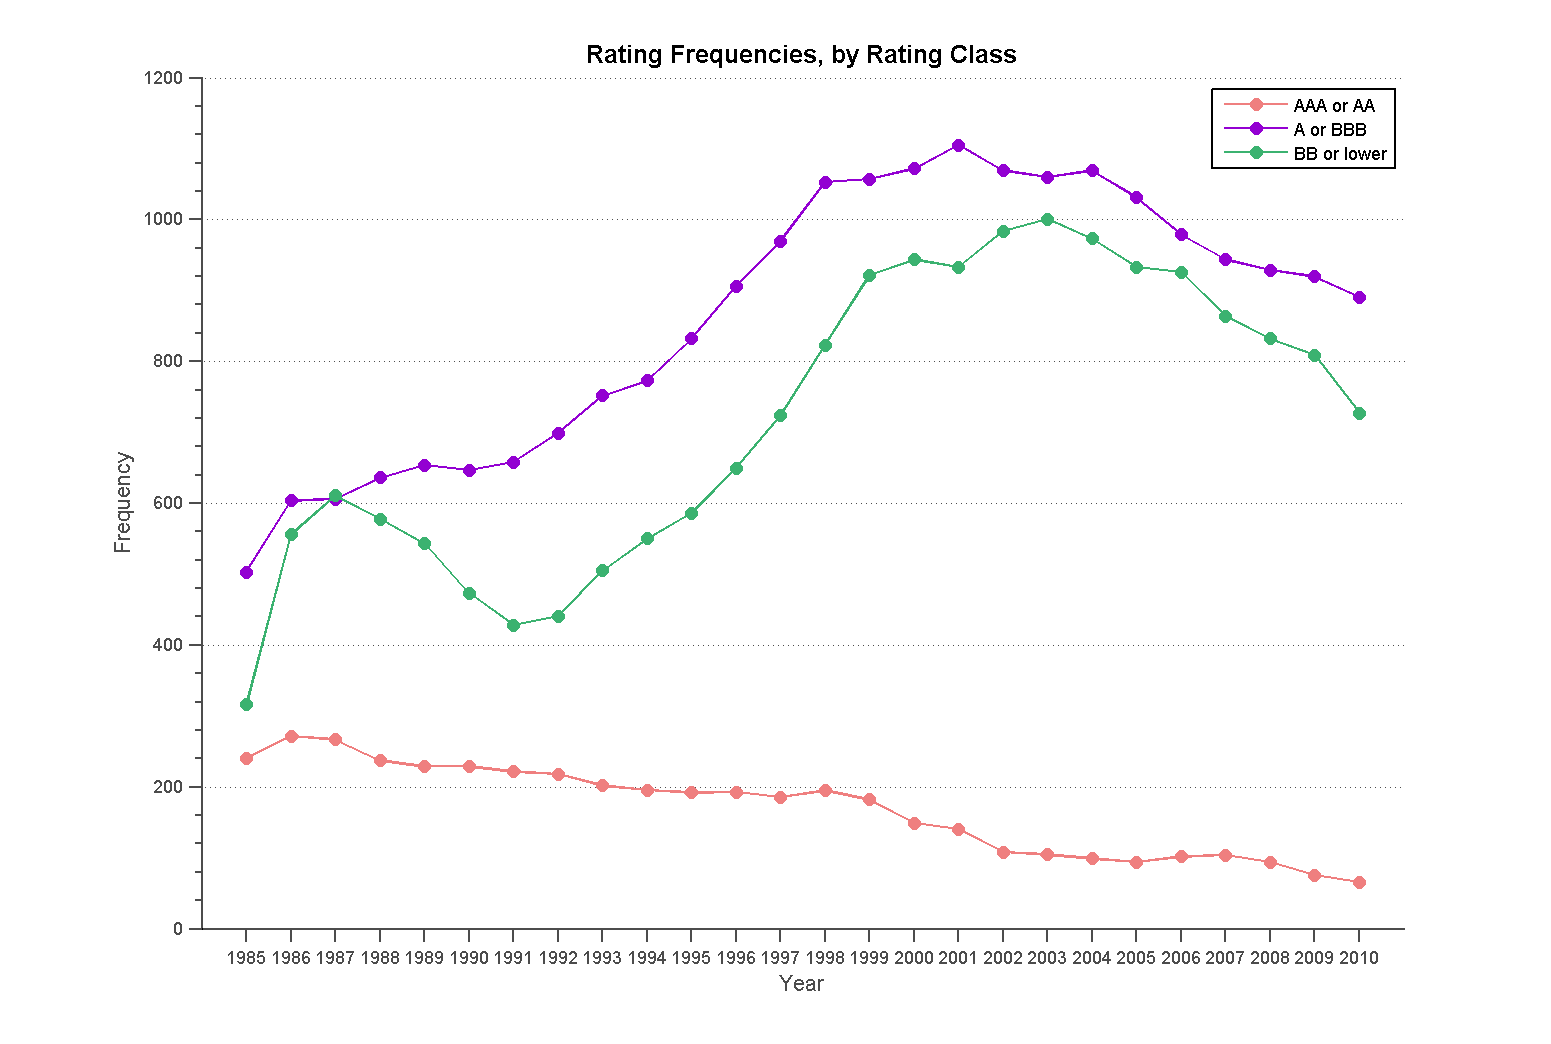
\includegraphics[width=\textwidth]{rate_freq.png}
\caption{Frequency of ratings by group: AAA or AA, A or BBB, and all speculative grade.}
\label{fig:count}
\end{figure}

\begin{figure}[ht]
\centering
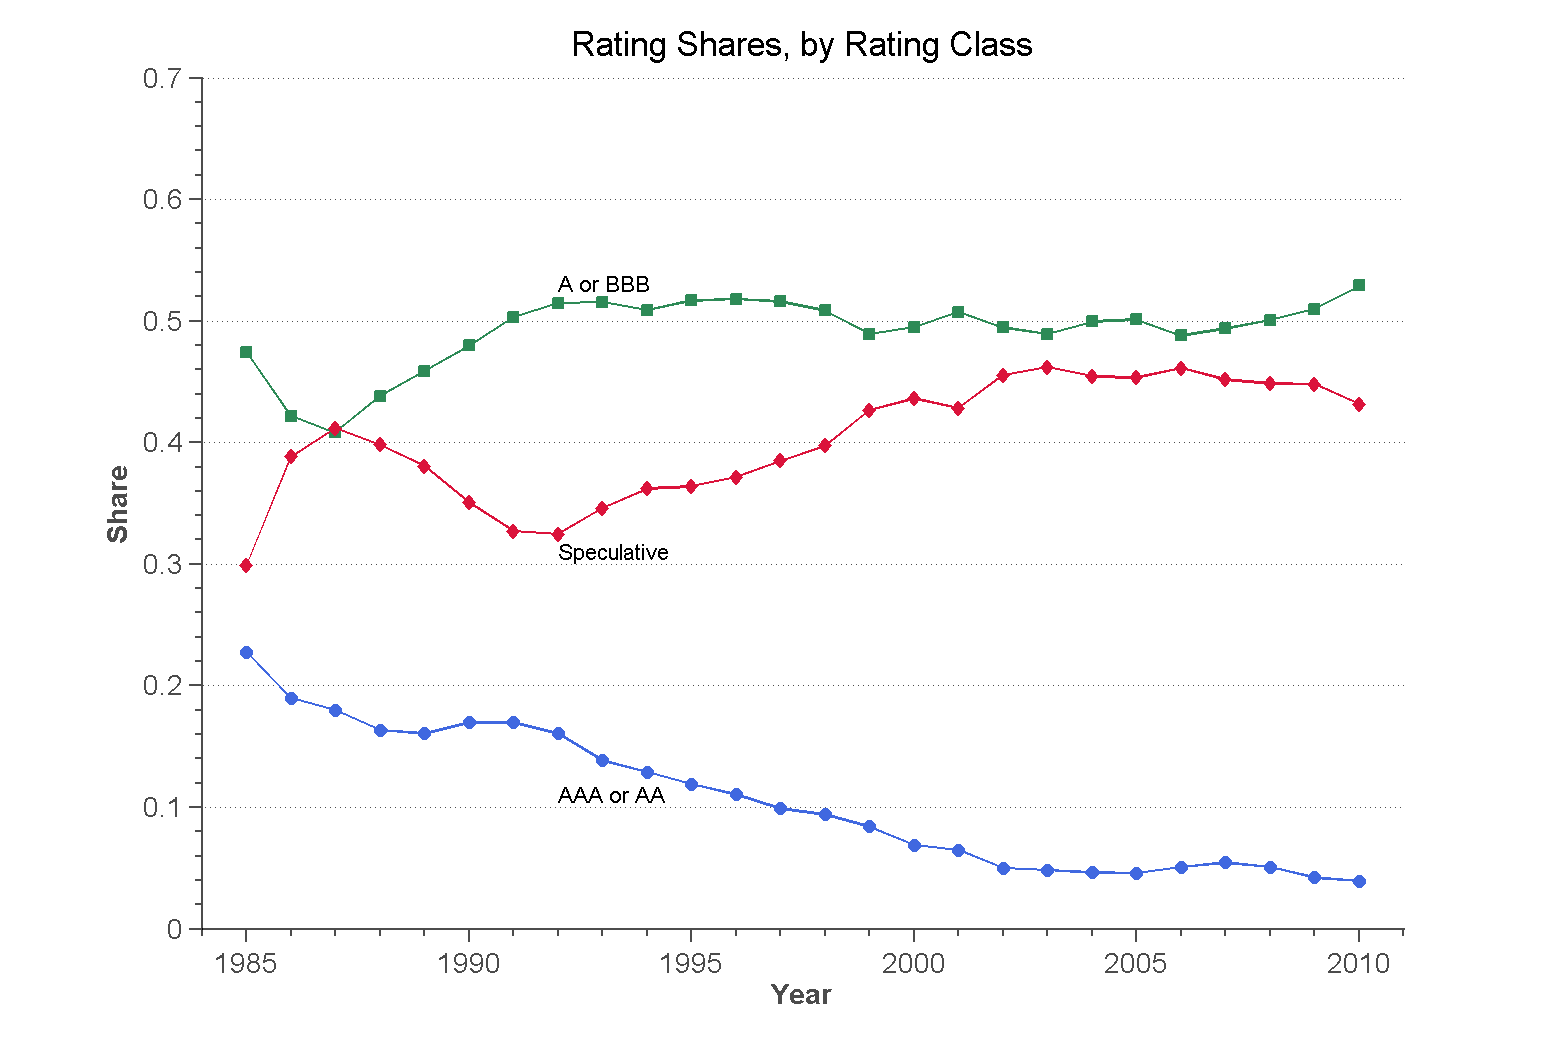
\includegraphics[width=\textwidth]{rate_share.png}
\caption{Share of ratings by group: AAA or AA, A or BBB, and all speculative grade.}
\label{fig:share}
\end{figure}

Why is the ratings distribution shifting towards more mediocre ratings? The answer to this question is important as bonds are now a larger share of corporate liabilities. In the Federal Reserve Board Flow of Funds Data, the share of total liabilities held in bonds grew by 26.5\% between 1985 and 2010. Corporations are increasingly choosing bond and equity financing over other securities and bank financing\footnote{The change in share of total corporate liabilities was 20.7\%, -76.7\%, and -67.1\% for equity, securities and bank financing, respectively.} Furthermore, the size the corporate bond market is massive; nonfinancial corporations had \$4,691.4 billion of outstanding bond debt in 2010.\footnote{\$5,286.0 billion oustanding at the end of 2012Q2, the most recent data available.} Considering the size and growth of this market, the underlying cause of the ratings shift may have a substantial effect on capital markets.

Credit ratings are obstensibly used by investors to determine how likely a firm is to default on its outstanding debt. Firms with AAA credit ratings are less likely to default than those rated AA, A, and so forth. On top of this, credit ratings are also a signal of the firm's general competence, as it is very difficult to achieve the highest ratings. As these ratings are useful to investors, firms will consult with ratings agencies prior to selling their debt.\footnote{Though it is possible to issue debt without consulting with a credit ratings agency, almost all firms do. Nevertheless, both Standard~\&~Poor's and Moody's will issue a rating regardless of the firm's paricipation.}

In part, the need for credit ratings is regulatory: many large, institutional investors are required to hold only investment grade bonds (BBB or higher). Additionally, it is difficult for firms to credibly relay this information directly to investors, and the auditing process would be very onerous for an individual investor. Thus the credit rating agencies are able to exploit some efficiencies of scale. There is a tradeoff for firms however: they must devote resources to non-productive ratings activities in order to satisfy the requirements of the credit rating agencies, on top of the fee for the rating service itself.\footnote{This is typically a percentage of the size of the bond issue.} For instance, a firm is required to hold cash on hand to satisfy the requirements for a particular rating. If credit ratings weren't required to sell corporate bonds, firms may be able to reallocate their resources to increase profits.

Considering the value of a credit rating, a natural question arises: why are the highly rated firms disappearing? I argue that firms are no longer willing to pay the cost to achieve high ratings. To this point:
\begin{quote}
``Scores of big companies have lost their AAA status in recent years as it became seen in board rooms as more of a straitjacket than a path to riches.''\attrib{Eric Dash, New York Times, August 2, 2011}
\end{quote}
To capture this change, I propose the following mechanism. As credit ratings have value as a signal of firm ``quality'' in the sense that they provide investors with information about the future performance of the firm, they are an alternative to other publicly available channels of firm information. These channels include SEC 10K filings, which contain pertinent financial data from public firms and are now provided electronically, and also include media such as the Wall Street Journal Online and Bloomberg. With the proliferation of this information, investors now have direct access to firm information which may convince them to purchase lower rated bonds. Firms no longer need to rely solely on a credit rating as a signal of their type as the demand for their bonds is now also dependent on this costless, public channel.

The topic was originally discussed in the financial press, from whom multiple answers have emerged. Besides firms unwillingness to pay for improved ratings, other suggestions include investors simply have a larger appetite for risk so are more willing to purchase lower rated bonds, and investors no longer place much stock in corporate bond ratings. Though seemingly disparate, I argue that these three answers are essentially the same. Firms will lower their rating and reduce the associated costs if they are able to sell their debt at a lower rating. This would be possible if the demand for lower investment grade bonds has increased relative to high investment grade bonds. In effect, there is lower demand for top ratings from both investors \emph{and} firms.

To formalize this story I construct a model that contains a ``peacock'' problem: the firm must divert resources to non-productive rating activities in order to improve its expected credit rating. Firms are endowed with a project and differ only in the probability that this project will pay off with the higher return. Both the credit rating and a costless public signal are correlated with the firm's type. This type is unknown to everyone, including the firm. As the firm learns something about its type from the public signal, this will influence the decision to invest in the rating process. Once this decision is made, a credit rating is formed. Knowing the public signal and the credit rating, investors then decide whether to invest in the firm's project. To capture the proliferation of information over the period in question, I increase the correlation of the public signal with a firm's type (the `accuracy' of the signal). Under general conditions, the resulting change in the distribution of credit ratings matches the change observed in the data.

The mechanism works as follows. Investors are unable to observe an individual firm's type but have access to credit ratings and the public signal. Firms with projects that have a higher expected payoff will be more likely to receive a high public signal and more likely to earn a high rating. The investors are then able to offer lower interest rates to those firms with higher ratings and signals. Additionally, a higher rating will increase the probability that a firm receives an investment. As the the accuracy of the signal increases, firms and investors learn more about the type of the firm, which may enduce firms to forego investing to achieve a high rating. In equilibrium, an increase in the accuracy of the public signal will result in fewer firms with high ratings and more firms with mediocre and low ratings.

The primary testable implication of the model is the increase in the dispersion of interest rates within a rating class. When the accuracy of the public signal is low, the interest rates given to two firms with the same rating and different signals will be closer than when the accuracy is high. In effect, the difference between the interest rates increases with the accuracy of the signal as investors are more sure that these firms have different underlying types. Using data from the \textit{Mergent Fixed Income Securities Databse}, I show that this pattern is borne out between 1990 to 2010. 

%Further testable implications include the pattern of firm switching between ratings and, with a more general version of the model, the implications for firm level and aggregate volatility in production.\footnote{The recent patterns in firm level and aggregate volatility are discussed in Comin \& Philippon (2006).} 

There are alternative explanations that need to be explored. One must consider that firms may be, in fact, more likely to default. That is, there exist fewer firms in 2010 with the same expected default rate as the AAA rated firms in 1985. It is very difficult to measure a change in default probabilities as the default rate for AAA and AA firms is very close to zero. A proxy for default probability is the leverage ratio, which is a measure of the indebtedness of firm relative to some form of its value, either assets or equity. It follows that a firm with a higher debt burden to value ratio will be more likely to default than one with either lower debt or higher firm value as the latter will find it easier to service its debt. I calculate and plot the average leverage ratios for different cohorts of AAA and AA rated firms over the relevant period in Figure~(\ref{fig:coh_lev}). The leverage ratios are roughly stable for each cohort. This indicates that higher levered firms do not seem to be driving the change in the ratings distribution.

It may be the case that the distribution of bond ratings has changed for reasons not related to firm behaviour. For instance, credit rating agencies may have changed the standards used to determine a firm's rating (or may be applying them differently), while the relevant measures of firm behaviour have remained constant. If this was the case the within rating average leverage ratios would either increase or decrease depending on whether that rating class has become relatively more or less prone to default. By computing the average leverage ratio within a rating by year, I show that this is not the case. Average leverage ratios have changed very little over the relevant period. The results can be seen in Figure~(\ref{fig:avg_lev}). 

Another possibility is that top rated firms are merging. To examine this I do two things. First, I show that the assets controlled by all AAA firms as a fraction of GDP is decreasing.\footnote{If AAA firms were merging, it may be the case that the assets controlled by all of these firms stayed roughly constant.} Second, as there are very few firms with AAA ratings, I can follow the cohort of AAA firms in 1985 to determine the evolution of their debt, including whether the debt rating changed, the debt was retired, or the firm merged with another. As can be seen in Table~(\ref{tab:mrg}), though some firms do merge when viewed over the entire horizon, for the most part the firms end up at a lower rating.

%Another possibility is that top rated firms are merging. To examine this I do two things. First, I calculate the assets controlled by all AAA firms as a fraction of GDP. If AAA firms were merging, it may be the case that the assets controlled by all of these firms stayed roughly constant. Figure~(\ref{fig:assets}) shows that this is not true; in fact, the assets controlled by AAA firms falls commensurate with the fall in the number of AAA firms themselves. Also, there is an increase in the assets controlled by firms in the ratings classes that are becoming more frequent. Second, as there are very few firms with AAA ratings, I can follow the cohort of AAA firms in 1985 to determine the evolution of their debt, including whether the debt rating changed, the debt was retired, or the firm merged with another. The results are shown in Table~(\ref{tab:mrg}). Though some firms do merge when viewed over the entire horizon, for the most part the firms end up at a lower rating.

In all markets, the rating system is designed to measure relative credit risk. The credit rating agencies (CRAs) assert that a rating does not measure absolute default probability and that a rating does not constitute investment advice. The purpose of this position is to ensure protection from liability claims and to continue their status as a Nationally Recognized Statistical Rating Organization (NRSRO). This designation is important as only ratings from such an organization may be used to satisfy legal obligations as to which debt may be held by large, institutional investors. An example of such an investor is a pension fund which is required to hold only investment grade debt.\footnote{Debt is considered investment grade if it has a rating of BBB or above. Debt rated BB or lower is deemed speculative grade or high yield.} Another example is any bank that has committed itself to the Basel Accords which specify a capital requirement based on the rating composition of the bank's assets.

Apart from the large U.S. banks, CRAs such as Standard\&Poor's, Moody's, and Fitch have suffered the most criticism in the wake of the recent financial crisis and the Great Recession. This criticism is perhaps justified in regards to how the CRAs rated structured finance products such as mortgage-backed securities and the credit default swaps based on these securities, but it is important to consider the different markets for ratings separately.\footnote{For articles concerned with these securities see, for instance, Bolton, Freixas \& Shapiro (2009) and He, Qian \& Strahan (2011) which are discussed later in this paper.} This is because the structure of the markets differs greatly, and thus the behaviour of CRAs will be different in each.

Though most academic work has focused on the CRA behaviour in the structured finance markets, Manso (2011) considers CRA behaviour in the market for corporate bonds. Where this paper studies an environment with a `passive' CRA, Manso (2011) shows the importance of feedback effects of rating changes when the CRA is able to choose the standards for a rating. The feedback effect begins with a rating adjustment which in turn affects the interest rate the firm is charged by the markets as the perceived default risk has changed. As the interest rate changes, the default probability will also change as the debt burden will increase or decrease with the change in interest rate. Thus a CRA which is more `lax' may be preferred to one with more stringent rating criteria. Another branch of the literature that concerns this work is credit rationing in the market for firm debt, which was introduced by Stiglitz~\&~Weiss (1981). The authors show that, under certain conditions, bank credit may be rationed between firms in markets with incomplete information. Bester (1985) extends the model to show that collateral may be used to screen firms and in this environment and at most one submarket will see credit rationing.

Skreta~\&~Veldkamp (2009) show that, as the complexity of the asset increases, the opportunity to ``shop for ratings'' also increases as it is more difficult to judge the default probability of the asset.\footnote{More specifically, when firms solicit multiple rating agencies the resulting difference in ratings will be larger across agencies if the rating produced is noisier. The rating will be noisier if the asset is more complex. Firms then choose the highest rating, and the resulting ratings distribution is ``inflated.''} This will then cause inflation in ratings. In a related paper, Bolton, Freixas \& Shapiro (2009) show that competition can also cause ratings inflation when investors cannot observe when a rating is produced but not published. Another feature of markets that may pervert CRA incentives is the concentration of issuers. He, Qian \& Strahan (2011) show that CRAs favoured large issuers during the recent financial crisis by giving their products higher ratings. This is because the primary source of CRA revenues is payments from issuers (referred to as an `issuer pays' model). In this paper I focus only on the market for corporate bonds which is not impacted by the above effects as the market is not dominated by a small number of issuers and corporate bonds are not complex assets. I further limit my focus to large firms.\footnote{I focus on large firms because I draw my sample from COMPUSTAT which includes only data on public firms. This is not a significant limitation as public firms are almost always large, and the corporate bond market is almost entirely comprised of bond issues from large firms. See Petersen \& Rajan (1995).}.

The paper proceeds as follows. Section~(\ref{sec:rat}) provides further detail about the change in the ratings distribution. The model is introduced and relevant results are shown in Sections~(\ref{sec:mod}) and (\ref{sec:res}). Section~(\ref{sec:cov}) shows the change in bond price dispersion. Section~(\ref{sec:dis}) discusses the empirical and analytical results. Section~(\ref{sec:con}) concludes.

\section{The Distribution of Ratings}
\label{sec:rat}
The firm data used in this project are from COMPUSTAT, including the ratings subset. This data covers all firms that file quarterly reports with the SEC. The ratings subset includes any firm which receives a rating from S\&P. I further restrict the sample to include only nonfinancial firms and firms not primarily owned by the federal government, as the process invovled in raising capital may vastly differ with that for nonfinancial firms. The sample includes 51,610 firm-year observations and 5,319 unique firms. 

The most natural reason for the number of AAA ratings to drop is that there are fewer firms with a default probability that is deserving of a AAA rating. That is, there exist fewer firms in 2010 with the same expected default rate as the AAA rated firms in 1985, assuming the required default rate for a AAA rating is the same. It is very difficult to measure a change in default probabilities as the default rate for AAA and AA firms is very close to zero. So, there may be no difference in the \emph{ex post} default rate despite a different expected default rate \textit{ex ante}. 

% ***need a lot more work here***
% \footnote{See XXX (YYY).} 
A useful proxy for default probability is the leverage ratio, which is a measure of the indebtedness of a firm relative to some form of its value, either assets or equity. It follows that a firm with a higher debt to value ratio will be more likely to default than one with either lower debt or higher firm value as the latter will find it easier to retire its debt. I calculate and plot the average leverage ratios for different cohorts of AAA and AA rated firms over the relevant period in Figure~(\ref{fig:coh_lev}). To do so, I calculate the ratio of total liabilities to total assets from individual components reported in COMPUSTAT, at an annual frequency.\footnote{Illiev \& Welch (2010) note that two correct alternatives exist, the liabilities to assets ratio and the debt to capital ratio. I compute both and find the same pattern in each.} The leverage ratios are roughly stable for each cohort. This indicates that more highly levered firms do not seem to be driving the change in the ratings distribution.

\begin{figure}[ht]
\centering
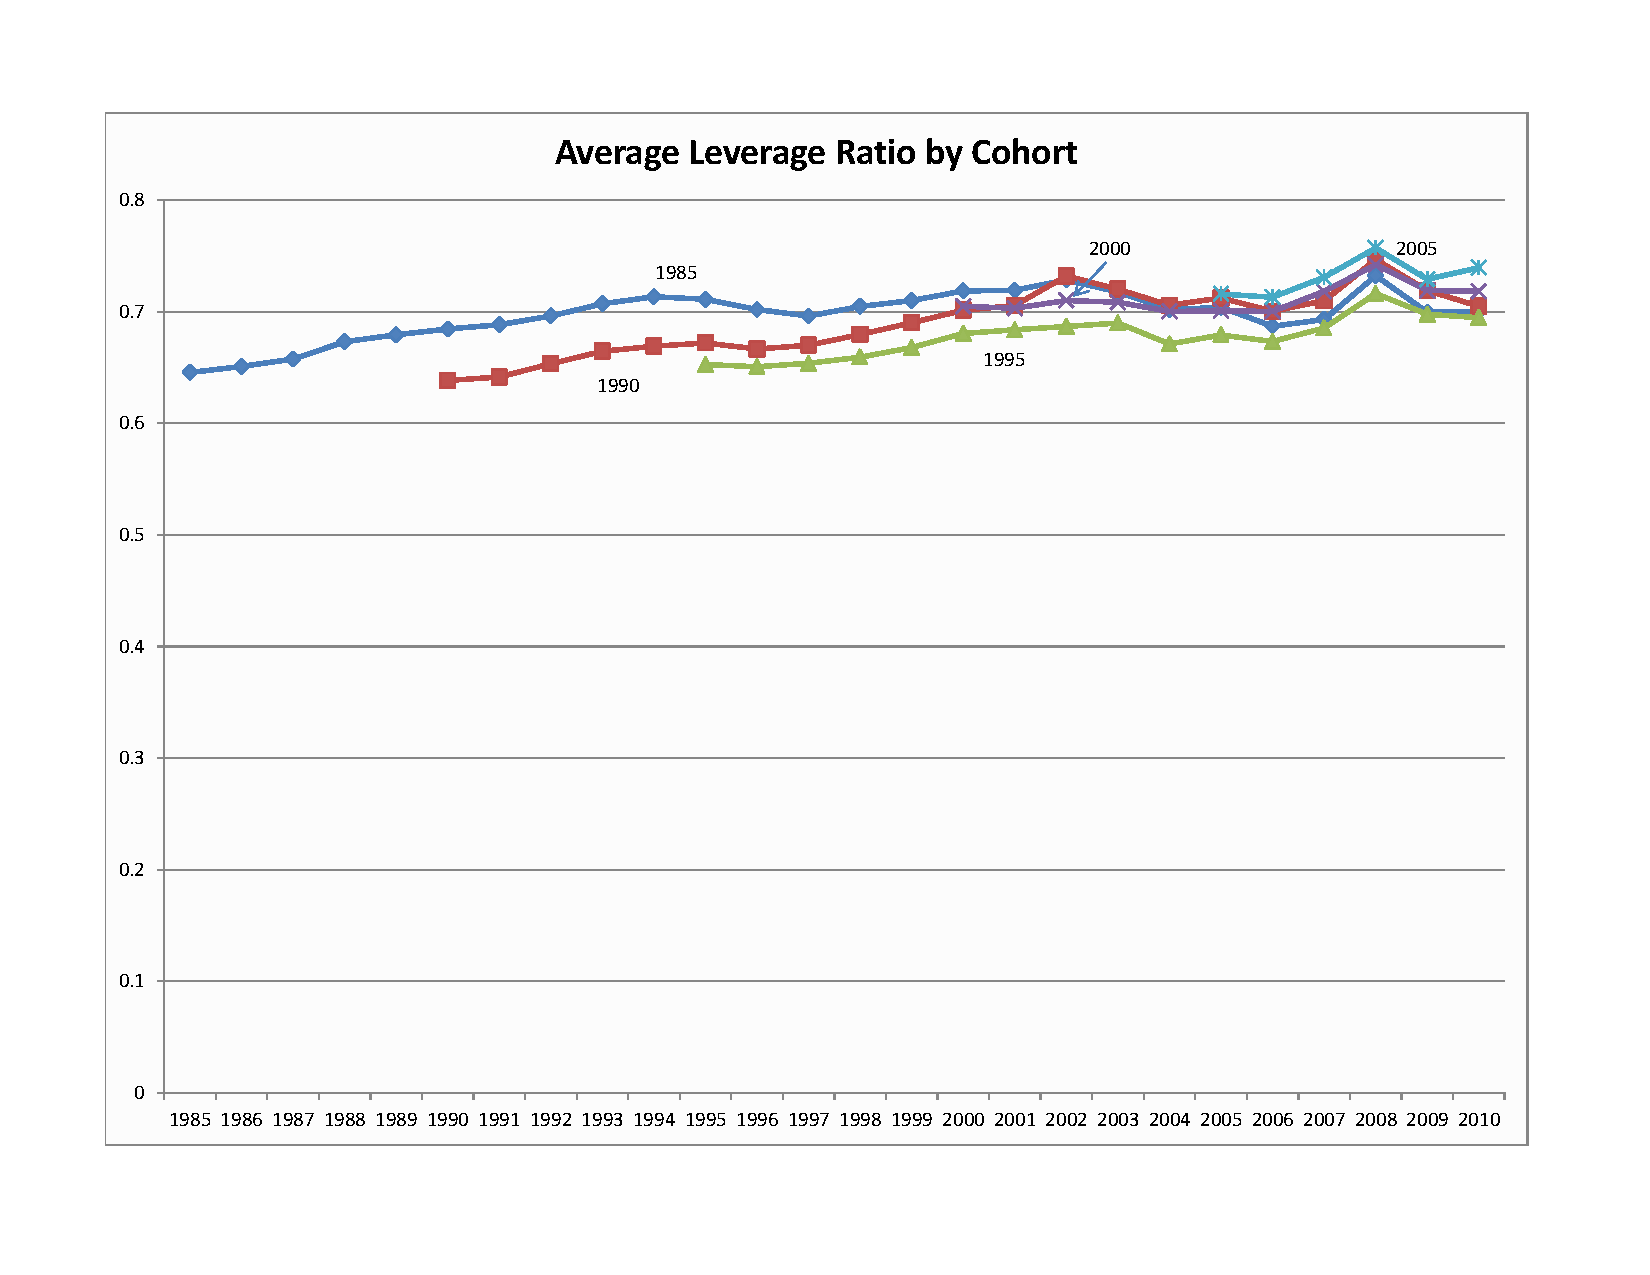
\includegraphics[width=\textwidth]{leverage_by_cohort_clr.pdf}
\caption{Within cohort average leverage ratios. A cohort is as all firms in the sample that were rated AAA or AA in the given year.}
\label{fig:coh_lev}
\end{figure}

It may be the case that the distribution of bond ratings has changed for reasons not related to firm behaviour. Primarily, CRAs may have changed the standards used to determine a firm's rating, while the relevant measures of firm behaviour have remained constant. If this was the case the within rating average leverage ratios would either increase or decrease depending on whether that rating class has become relatively more or less prone to default. By computing the average leverage ratio within a rating by year, I show that this is not the case. Average leverage ratios have changed very little over the relevant period. The results can be seen in Figure~(\ref{fig:avg_lev}). 

\begin{figure}[ht]
\centering
	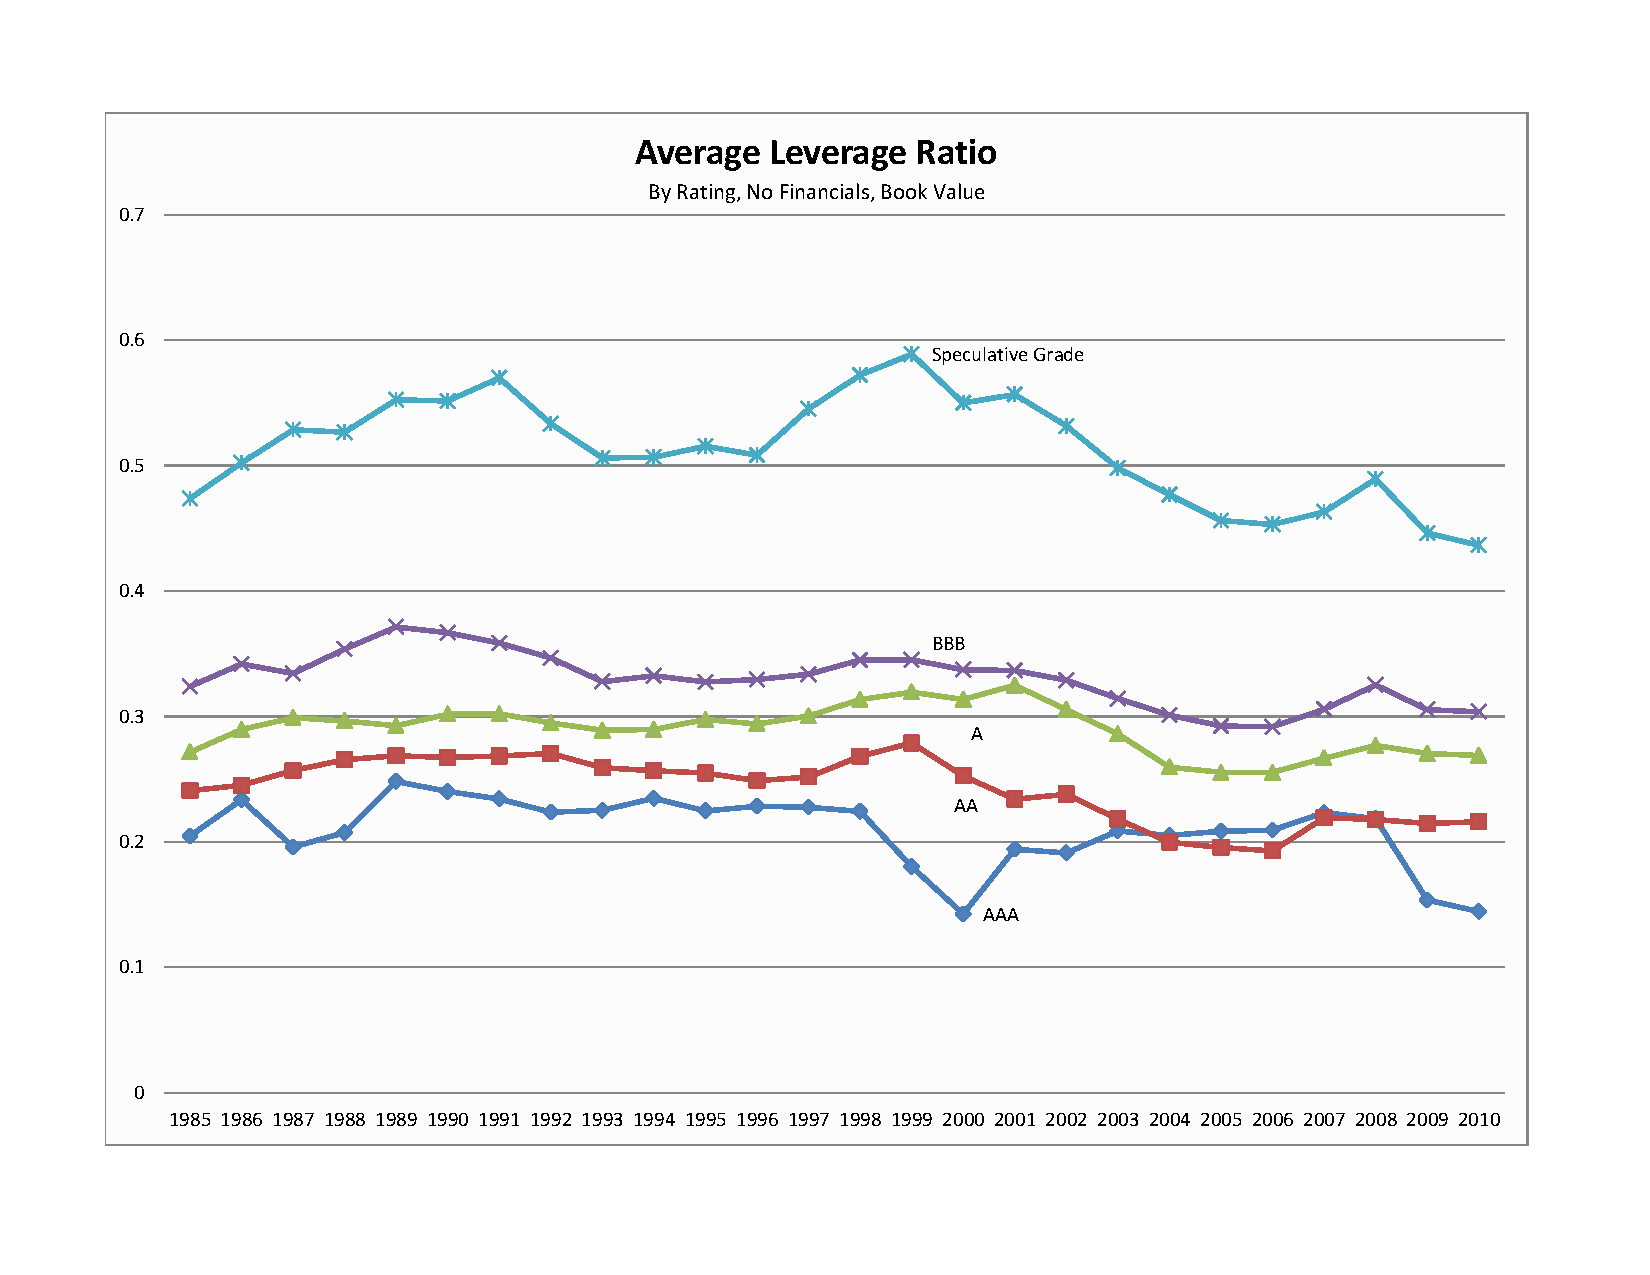
\includegraphics[width=\textwidth]{avg_leverage_bv_nofin.pdf}
	\caption{Within rating average leverage ratios.}
	\label{fig:avg_lev}
\end{figure}

Another possibility is that highly rated firms are merging. This would imply a decrease in the number of highly rated firms, without a significant drop in the total assets controlled by these firms. By aggregating the assets over ratings and normalizing the levels by dividing by GDP, I show that the share of assets controlled by AAA and AA rated firms has dropped significantly. The decrease in asssets held by AAA and AA rated firms is comensurate with the decrease in the number of AAA and AA rated firms. Also, there is an increase in the assets controlled by firms rated A, BBB, or lower, again matching the change in the rating distribution. These series can be seen in Figure (\ref{fig:assets}). 

To further validate this claim, in Table (\ref{tab:mrg}) I follow the 1985 cohort of AAA rated firms. Though 6 of the 34 firms with a AAA rating did eventually exit the sample through merger, a majority of the firms arrived at the end of the sample with a lower credit rating. In fact, all but one of the firms that merged over this period were involved in the conglomeration of regional telecommunications companies into the national entities in operation today.

\begin{figure}[ht]
\centering
	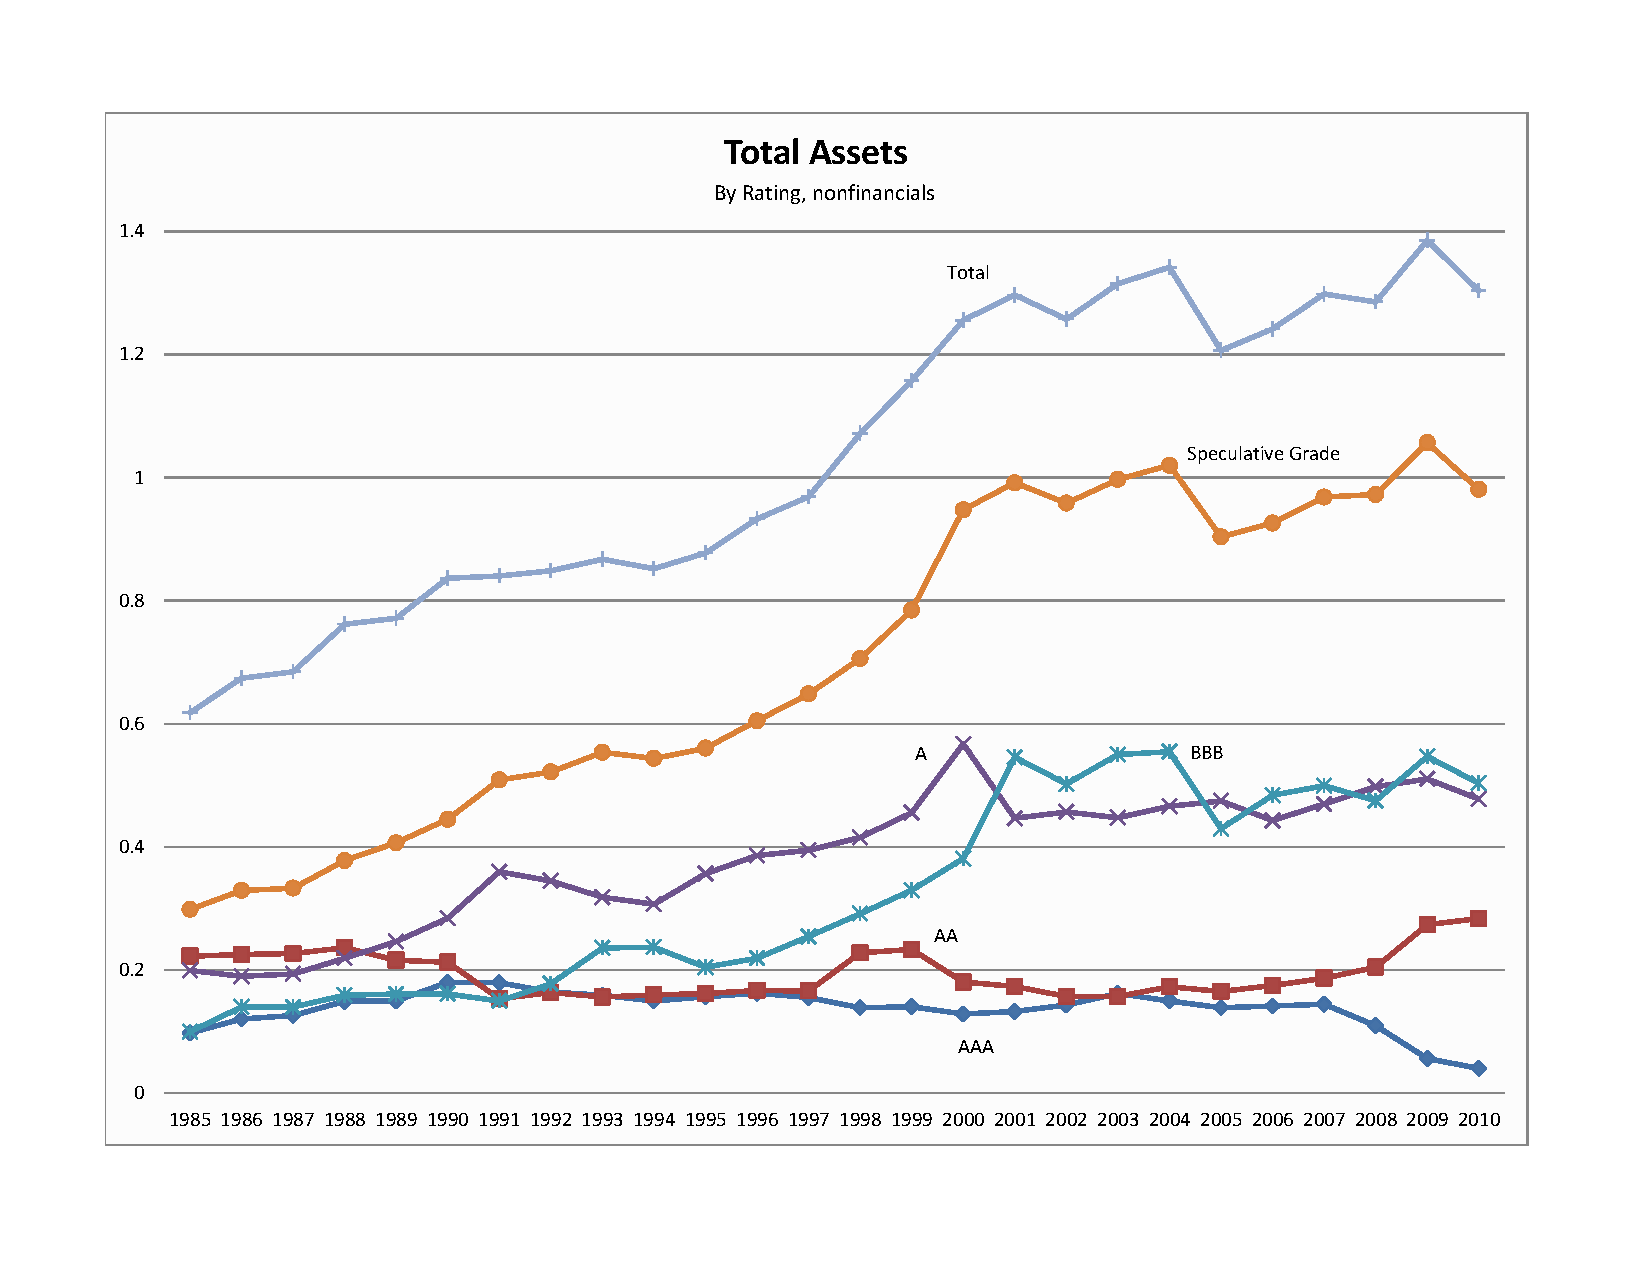
\includegraphics[width=\textwidth]{assets_nf.pdf}
	\caption{Assets controlled by each rating class, as a fraction of GDP.}
	\label{fig:assets}
\end{figure}

\begin{table}\centering
\begin{tabular}{l *{6}r}
\toprule
  	& 1985  & 1990  & 1995  & 2000  & 2005  & 2010\\ \midrule
AAA  	& 34  	& 26  	& 17  	& 8  	& 4  	& 1\\
AA  	& 0  	& 4  	& 8  	& 3  	& 6  	& 8\\
A  	& 0  	& 1  	& 3  	& 9  	& 6  	& 7\\
BBB  	& 0  	& 0  	& 1  	& 2  	& 3  	& 3\\
B  	& 0  	& 1  	& 1  	& 0  	& 0  	& 0\\
Merged 	& 0  	& 1  	& 2  	& 6  	& 6  	& 6\\
Retired	& 0  	& 1  	& 2  	& 6  	& 9  	& 9\\ 
\bottomrule
\end{tabular}
\caption{Evolution of circa 1985 AAA firms (also include circa 85 AA firms?)}
\label{tab:mrg}
\end{table}
% (also include circa 85 AA firms?)
A final concern that I have addressed is that, although the distribution of ratings may be changing due to some previously unexplored effect, ratings are now insignificant as bonds make a smaller portion of firm financing. This does not seem to be the case, however. Using the Federal Reserve Board of Governors Flow of Funds dataset, I calculate that the share of corporate bonds to total liabilities has increased by 26\% from 1985 to 2010 for all nonfarm, nonfinancial corporations. Of the other broad classes of financing, equity grew by 20.7\%, while other securities and bank financing decreased by 76.7\% and 67.1\%, respectively.

\section{Model}
\label{sec:mod}
The aim of the model is to capture the change in the way investors obtain information relevant to their purchase of corporate bonds. Obtaining relevant information directly from the firm is costly for an individual investor, if it is possible at all, whereas rating agencies distribute a summary of this information in the form of a credit rating. In order to attain a higher rating, firms must devote resources to non-productive ratings activities, such as increasing their cash at hand. As the access to financial information has increased for investors, through channels such as electronic distribution of SEC 10K filings and other sources discussed above, there is now a direct channel between firms and investors. I model this channel as a noisy public signal that is correlated with the probability that a firm's project will result in the higher return, which I call the firm's type. 

This section continues with an outline of the environment which describes the players, timing, and information flows. More detail is then provided about the role of public signals and credit ratings. The firm and investor problems follow. The equilibrium concept is then defined, along with the solution to the firm's problem and the investor's decision rule.

\subsection{Environment}
Firms are endowed with a project which will have either a low or high return. The probability of the high return is referred to as the firm's type, $\theta \epsilon \{g,b\}$, is unknown to all. First, a public signal, $\nu \epsilon \{h,l\}$, which is correlated with the firm's type is observed by all. The firm then chooses the amount of resources it devotes to non-productive rating activities, $i  \epsilon [0,1]$, knowing the public signal but not their type. Let $c(i)$ be the cost investing $i$. This investment will increase the probability that the firm receives a high credit rating and lower the probability is receives a low credit rating.

A credit rating, $\kappa \epsilon \{A,B,C\}$, which is also correlated with the firm's type, is then produced by a passive credit rating agency, and observed by all. The distribution of credit ratings depends on both $\theta$ and $i$. After observing $\nu$ and $\kappa$, investors decide whether to purchase the firm's debt at the market interest rate, $R(\kappa,\nu)$. The outcome of the project is then realized and debts are paid.

To make the investment decision non-trivial I assume that probability of the higher return is such that the expected return to low-type projects is lower than the borrowing cost required to satisfy investors. As such, firms would rather walk away from a succesful project than pay back investors. Anticipating this, investors will choose not to invest in firms that are known to be `low' type.

\subsection{Credit Ratings and Public Signals}
The credit rating agency assigns a rating, $\kappa\epsilon\left\{A,B,C\right\}$, to each firm. The probability that a firm receives a given rating is determined by its type, $\theta$, and the amount of resources that the firm chooses to invest in the ratings process, $i$. Let $\pi_{\kappa}(\theta,i)$ be the probability that a firm of type $\theta$ that invested $i$ receives rating $\kappa$. I assume that $\pi_{A}(\theta,i)$ is increasing in $i$ for every $\theta$ whereas both $\pi_{B}(\theta,i)$ and $\pi_{C}(\theta,i)$ are decreasing in $i$. Thus, as firms increase $i$ they increase the probability that they receive a high rating. I assume the rating production functions are linear and obey the following conditions:
\begin{align} 
\label{a1}\pi_{A}(g,i)>\pi_{A}(b,i) \forall i \\
\label{a2}\pi_{C}(g,i)<\pi_{C}(b,i) \forall i 
\end{align}
Simply put, these assumptions rule out the possibility of equilibria in which the pool of $A$-rated firms is more likely to default on average than the pool of $C$-rated firms. In essence this ensures that the ratings are informative, in that higher ratings are correlated with lower default rates.

%justify this
The functional forms chosen are as follows:
\begin{align*}
	\pi_{A}(g,i) & = \sigma^{g}_{1} + (\sigma^{g}_{2}+\sigma^{g}_{3})i\\
	\pi_{A}(b,i) & =         (\sigma^{b}_{2}+\sigma^{b}_{3})i\\
	\pi_{B}(g,i) & =          \sigma^{g}_{2}(1-i )\\
	\pi_{B}(b,i) & =          \sigma^{b}_{2}(1-i )\\
	\pi_{C}(g,i) & =          \sigma^{g}_{3}(1-i )\\
	\pi_{C}(b,i) & = \sigma^{b}_{1} +  \sigma^{b}_{3}(1-i ),
\end{align*}
where
\begin{align*}
\sigma^{g}_{1}+\sigma^{g}_{2}+\sigma^{g}_{3} & =1\\
\sigma^{b}_{1}+\sigma^{b}_{2}+\sigma^{b}_{3} & =1.
\end{align*}
(\ref{a1}) and (\ref{a2}) imply that $g_{1}>0$ and $b_{1}>0$.

The noisy public signal, $\nu\epsilon \{H,L\}$, that may be correlated with a firm's type, is seen by investors and firms. The distribution of $\nu$ is as follows: $Pr \{\medmath{H} | \medmath{g} \}=Pr \{\medmath{L} | \medmath{b} \}=\omega$ and $Pr \{\medmath{L} | \medmath{g} \}=Pr \{\medmath{H} | \medmath{b} \}=1-\omega$. One can interpret $\omega$ as the probability that the public signal is accurate, i.e.\ the probability that good firms get high public signals, and bad firms get low public signals. As constructed, if $\omega > 1/2$ the public signal is informative in that signal $H$ is correlated with type $g$ and $L$ with $b$.\footnote{Note that, if $\omega<1/2$, the public signal is still correlated with the firm's type. In this case, the high public signal would be positively correlated with bad firms, and vice versa.}

\subsection{Firms}
Firms differ in their unobservable type, $\theta \epsilon \left\{g,b\right\}$. The distribution of $\theta$ is as follows: $Pr\{g\}=\lambda$ and $Pr\{b\}=1-\lambda$. Firms are endowed with a risky project that will return $y$ with probability $\gamma_{\theta}$, where $\gamma_{g}>\gamma_{b}$, and 0 otherwise. The firm must receive an investment of fixed size $d=1$ to start the project. The distribution of types is common knowledge. 

The timing for firms is as follows. The firm first observes its noisy signal, $\nu$, and then chooses the level of resources to invest in rating activities, $i$, in order to maximize the expected value of the project net of borrowing costs. At this point the firms do not know their rating and thus the expectation is taken over both the probability the project will return $y$ given $\nu$ and the distribution of ratings given $\nu$ and $i$ as the rating will influence the borrowing cost $R(\kappa,\nu)$.

Given gross interest rates $R(\kappa,\nu)$, the firm's problem is the following:
\begin{align}
\label{eq:FP} V(\nu)=\max_{i} & -c(i)+\textup{E}_{\theta,h} [ \mathbbm{1}(\kappa,\nu) (y - R(\kappa,\nu)|\nu ) ]\\
\textup{subject to: } & i\epsilon [0,1] \nonumber
\end{align}
I assume $c(i)$ is increasing, $c'(0)=0$ and $c'(1)=\infty$. The indicator function $\mathbbm{1}(\kappa,\nu)$ is equal to 1 when an investment is received, and 0 otherwise. It is allowed to depend on $\kappa$ and $\nu$ as both are available to investors when they make their decision to invest. The benefits of a higher $i$ are lower expected borrowing cost ($R(\kappa,\nu)$) as the expected rating is higher, and an increased probability of receving an investment. The firm weighs these benefits against the cost of investing in the rating process, $c(i)$. As firms do not observe their type, the public signal determines the level of investment that balances these expected benefits and costs. Thus, firms that receive the low public signal $L$ may still be $g$-type and there is a benefit to investing in the rating. Conversely, firms that receive the high public signal $H$ have some assurance of their being a $g$-type, but may in fact be $b$-type. 

\subsection{Firms}
Firms differ in their unobservable type, $\theta \epsilon \left\{G,B\right\}$. The distribution of $\theta$ is as follows: $Pr\{G\}=\lambda$ and $Pr\{B\}=1-\lambda$. Firms are endowed with a risky project that will return $y$ with probability $\gamma_{\theta}$, where $\gamma_{G}>\gamma_{B}$, and 0 otherwise. The firm must receive an investment of fixed size $d=1$ to start the project. The distribution of types is common knowledge. 

The timing for firms is as follows. The firm first observes its noisy signal, $\nu$, and then chooses the level of resources to invest in rating activities, $i$, in order to maximize the expected value of the project net of borrowing costs. At this point the firms do not know their rating and thus the expectation is taken over both the probability the project will return $y$ given $\nu$ and the distribution of ratings given $\nu$ and $i$ as the rating will influence the borrowing cost $R(\kappa,\nu)$.

Given gross interest rates $R(\kappa,\nu)$, the firm's problem is the following:
\begin{align}
\label{eq:FP} V(\nu)=\max_{i} & -c(i)+\textup{E}_{\theta,h} [ \mathbbm{1}(\kappa,\nu) (y - R(\kappa,\nu)|\nu ) ]\\
\textup{subject to: } & i\epsilon [\underline{i},\bar{i}] \nonumber
\end{align}
I assume $c(i)$ is increasing, $c'(0)=0$ and $c'(1)=\infty$. The indicator function $\mathbbm{1}(\kappa,\nu)$ is equal to 1 when an investment is received, and 0 otherwise. It is allowed to depend on $\kappa$ and $\nu$ as both are available to investors when they make their decision to invest. The benefits of a higher $i$ are lower expected borrowing cost ($R(\kappa,\nu)$) as the expected rating is higher, and an increased probability of receving an investment. The firm weighs these benefits against the cost of investing in the rating process, $c(i)$. As firms do not observe their type, the public signal determines the level of investment that balances these expected benefits and costs. Thus, firms that receive the low public signal $L$ may still be a $G$-type there is a benefit to investing in the rating. Conversely, firms that receive the high public signal $H$ have some assurance of their being a $G$-type, but may in fact be $B$-type. 

\subsection{Investors}
Investors are endowed with 1 unit of investment capital which they can invest in either firm debt at the market interest rate, $R(\kappa,\nu)$, or government debt at the risk-free interest rate, $r$. Before making this decision, investors observe a credit rating, $\kappa$, and public signal, $\nu$, from the firm. If the investor chooses to purchase firm debt,she will then be repaid $R(\kappa,\nu)$ at the end of the period if the firm honours its debt. Investors face no barriers to entry in the market for debt and investment capital is available in perfectly elastic supply. The expected investor return to firm debt rated $\kappa$ with signal $\nu$ is:
% As capital markets are perfectly competitive, the expected investor return to firm debt rated $\kappa$ with signal $\nu$ is equal to the return to government debt:
\begin{equation}
\textup{E}_{\theta} [R(\kappa,\nu)|\kappa,\nu ].
\end{equation}

\subsection{Equilibrium}

An equilibrium is a set of interest rates, $\mathbf{R}^{*}=\{ R^{*}(\kappa,\nu)\}_{\kappa\epsilon\{A,B,C\}}^{\nu\epsilon\{H,L\}}$, and rating investment allocations, $\{i^{*}_{\nu}\}^{\nu\epsilon\{H,L\}}$ such that:
\begin{enumerate}
	%\setlength{\itemindent}{0.8cm}
	\item given $\mathbf{R}^{*}$, $i^{*}_{\nu}$ solves (\ref{eq:FP});
	\item Investors are perfectly competitive: $\textup{E}_{\theta} [R^{*}(\kappa,\nu)|\kappa,\nu ] = r \,\, \forall \kappa, \nu$.
\end{enumerate}

\subsection{Solution to the Firm's Problem}
Taking first order conditions and solving for $i$:
\begin{align}
i^{*}(H) = & (c')^{-1}\sum_{\kappa \epsilon \{A,B,C\}} \frac{\omega\lambda\gamma_{g}\pi_{\kappa}'(g)+(1-\omega)(1-\lambda)\gamma_{b}\pi_{\kappa}'(b)}{\omega\lambda+(1-\omega)(1-\lambda)}(y-R^{*}(\kappa,H))\mathbbm{1}(\kappa,H)\\
i^{*}(L) = & (c')^{-1}\sum_{\kappa \epsilon \{A,B,C\}} \frac{(1-\omega)\lambda\gamma_{g}\pi_{\kappa}'(g)+\omega(1-\lambda)\gamma_{b}\pi_{\kappa}'(b)}{(1-\omega)\lambda+\omega(1-\lambda)}(y-R^{*}(\kappa,L))\mathbbm{1}(\kappa,L)
\end{align}
where $(c')^{-1}$ is the inverse marginal cost function.

\subsection{Investor's Decsion}
Invest if $y>R^{*}(\kappa,\nu)$.

\subsection{Interest Rates}
Considering the free entry condition for firms, the following are the equilibrium interest rates.
\begin{align}
R^{*}(\kappa,\nu) = & \frac{r}{\textup{E}_{\theta}(\gamma_{\theta}|\kappa,\nu)}\\
R^{*}(\kappa,\medmath{H}) = & r\frac{\omega\lambda\pi_{\kappa}(g,i^{*}(\medmath{H}))\gamma_{g}+(1-\omega)(1-\lambda)\pi_{\kappa}(b,i^{*}(\medmath{H}))\gamma_{b}}{\omega\lambda\pi_{\kappa}(g,i^{*}(\medmath{H}))+(1-\omega)(1-\lambda)\pi_{\kappa}(b,i^{*}(\medmath{H}))}\\
R^{*}(\kappa,\medmath{L}) = & r\frac{(1-\omega)\lambda\pi_{\kappa}(g,i^{*}(\medmath{L}))\gamma_{g}+\omega(1-\lambda)\pi_{\kappa}(b,i^{*}(\medmath{L}))\gamma_{b}}{(1-\omega)\lambda\pi_{\kappa}(g,i^{*}(\medmath{L}))+\omega(1-\lambda)\pi_{\kappa}(b,i^{*}(\medmath{L}))}
\end{align}

\section{Results}
\label{sec:res}%

In this section I first show that firms will decrease $i$ when the accuracy of the public signal increases. This is due to the with rating class compositional change that occurs when firms change $i$. This result leads to Proposition~(\ref{pr:dist}), the main result of the paper. This states that an increase in the accuracy of the public signal will decrease the number of firms with an $A$ rating, while increasing the number of firms with a $B$ or $C$ rating, a shift which matches the real-life shift described above. 
%To test the viability of my conjecture, that an increase in information proliferation has the shift in the ratings distribution, I increase the accuracy of the noisy public signal. Proposition~\ref{pr:pi} 
\begin{proposition}
\label{pr:pi}
The equilibrium investment in the ratings process for firms with signal $\nu$, $i^{*}_{\nu}$, is decreasing in public signal accuracy, $\omega$.
\end{proposition}

\begin{proof}
Suppose not. Then for some $\omega$, $i^{*}_{\nu}$ increases in $\omega$. This implies that the probability of getting an $A$ ($C$) rating is increasing (decreasing) for firms with signal $\nu$. The relevant rating production functions are as follows:
\begin{align*}
\textup{Pr}\left ( \medmath{A} | \medmath{g,\nu} \right) &= \sigma^{g}_{1} + (\sigma^{g}_{2}+\sigma^{g}_{3})i_{\nu}\\
\textup{Pr}\left ( \medmath{A} | \medmath{b,\nu} \right) &= (\sigma^{b}_{2}+\sigma^{b}_{3})i_{\nu}\\
% \textup{Pr}\left ( \medmath{b} | \medmath{g,\nu} \right) &= g_{2}(1-x_{\nu})\\
% \textup{Pr}\left ( \medmath{b} | \medmath{b,\nu} \right) &= b_{2}(1-x_{\nu})\\
\textup{Pr}\left ( \medmath{C} | \medmath{g,\nu} \right) &= \sigma^{g}_{3}(1-i_{\nu})\\
\textup{Pr}\left ( \medmath{C} | \medmath{b,\nu} \right) &= \sigma^{b}_{1} +  \sigma^{b}_{3}(1-i_{\nu}).
\end{align*}

Most directly relevant to investors is the probability that a firm is a certain type, conditional on the observed rating and signal. Employing Bayes' rule and the law of total probability, the probability that a firm is type $\theta$ conditional on observing $\kappa$ and $\nu$ is:
\begin{equation*}
\textup{Pr}(\medmath{\theta}|\medmath{\kappa,\nu})=\frac{\textup{Pr}(\medmath{\kappa}|\medmath{\nu,\theta})\textup{Pr}(\medmath{\nu}|\medmath{\theta})\textup{Pr}(\medmath{\theta})}{\textup{Pr}(\medmath{\kappa}|\medmath{\nu,\theta})\textup{Pr}(\medmath{\nu}|\medmath{\theta})\textup{Pr}(\medmath{\theta})+\textup{Pr}(\medmath{\kappa}|\medmath{\nu,\bar{\theta}})\textup{Pr}(\medmath{\nu}|\medmath{\bar{\theta}})\textup{Pr}(\medmath{\bar{\theta}})}.
\end{equation*}
In particular, the relevant probabilities are:
\begin{align*}
\textup{Pr}(\medmath{g}|\medmath{A,H})&=%
\frac{\pi_{A}(g,i_{H})\omega\lambda}{\pi_{A}(g,i_{H})\omega\lambda+\pi_{A}(b,i_{H})(1-\omega)(1-\lambda)},\\
\textup{Pr}(\medmath{g}|\medmath{A,L})&=%
\frac{\pi_{A}(g,i_{L})(1-\omega)\lambda}{\pi_{A}(g,i_{L})(1-\omega)\lambda+\pi_{A}(b,i_{L})\omega(1-\lambda)},\\
\textup{Pr}(\medmath{g}|\medmath{C,H})&=%
\frac{\pi_{C}(g,i_{H})\omega\lambda}{\pi_{C}(g,i_{H})\omega\lambda+\pi_{C}(b,i_{H})(1-\omega)(1-\lambda)},\\
\textup{Pr}(\medmath{g}|\medmath{C,L})&=%
\frac{\pi_{C}(g,i_{L})(1-\omega)\lambda}{\pi_{C}(g,i_{L})(1-\omega)\lambda+\pi_{C}(b,i_{L})\omega(1-\lambda)}.
\end{align*}
% \begin{align*}
% \textup{Pr}(\medmath{g}|\medmath{A,H})&=%
% \frac{(g_{1}+(g_{2}+g_{3})i_{H})\omega\lambda}{(g_{1}+(g_{2}+g_{3})i_{H})\omega\lambda+(b_{2}+b_{3})i_{H}(1-\omega)(1-\lambda)},\\
% \textup{Pr}(\medmath{g}|\medmath{A,L})&=%
% \frac{(g_{1}+(g_{2}+g_{3})i_{H})(1-\omega)\lambda}{(g_{1}+(g_{2}+g_{3})i_{H})(1-\omega)\lambda+(b_{2}+b_{3})i_{H}\omega(1-\lambda)},\\
% \textup{Pr}(\medmath{g}|\medmath{C,H})&=%
% \frac{g_{3}(1-i_{H})\omega\lambda}{g_{3}(1-i_{H})\omega\lambda+(b_{1}+b_{3}(1-i_{H}))(1-\omega)(1-\lambda)},\\
% \textup{Pr}(\medmath{g}|\medmath{C,L})&=%
% \frac{g_{3}(1-i_{H})(1-\omega)\lambda}{g_{3}(1-i_{H})(1-\omega)\lambda+(b_{1}+b_{3}(1-i_{H}))\omega(1-\lambda)}.
% \end{align*}
Under assumptions \ref{a1} and \ref{a2}, each of these probabilities is decreasing in $i$.\footnote{See Appendix~(\ref{app:pr:pi}).} Thus, the proportion of firms with an $A$ or $C$ rating and an $H$ or $L$ signal that are $g$-type will be lower if firms increase $i$. Conversely, the proportion that are $b$-type will be higher.

As the pool of firms with an $A$ or $C$ rating and $\nu$ signal now contains proportionately less of type $g$ and more type $b$ firms, the expected default rate of the pool will increase. The corresponding change in the interest rate is:
\begin{align}
\frac{\partial \textup{R}^{*}(\medmath{\kappa,H})}{\partial i^{*}_{\nu}} &= 
\frac{r\omega\lambda(1-\omega)(1-\lambda)[\kappa(\medmath{G,i^{*}_{\nu}})\kappa' (\medmath{b})-\kappa (\medmath{B,i^{*}_{\nu}})\kappa' (\medmath{g})](\gamma_{g}-\gamma_{b})}{(\textup{Pr}(\medmath{g,\nu,\kappa}|\medmath{i^{*}_{\nu}})\gamma_g + \textup{Pr}(\medmath{B,\nu,\kappa}|\medmath{i^{*}_{\nu}})\gamma_b)^2},
\end{align}
where $\pi_{\kappa}(\theta,i)$ is the probability of receiving rating $\kappa$ at type $\theta$ and investment $i$, and $\pi_{\kappa}'(\theta)$ is the derivative of $\pi_{\kappa}$ with respect to $i$. This expression is positive, indicating that $\textup{R}^{*}(\medmath{\kappa}|\medmath{\nu})$ is increasing in $i^{*}_{\nu}$ for $\kappa$ equal to $A$ or $C$. The interest rate increases because the proportion of type $g$ firms is decreasing (and thus that of $b$ types is increasing) in the pool of $A$ or $C$-rated, $\nu$-signal firms.\footnote{This is true as $\frac{\kappa'(\medmath{g})}{\pi_{\kappa}(\medmath{g,i})}<\frac{\pi_{\kappa}'(\medmath{b})}{\pi_{\kappa}(\medmath{b,i})}$ for $\kappa\epsilon\left\{A,C\right\}$, which holds whenever $g_{1}>0$ and $b_{1}>0$, respectively.} So, a random $A$ or $C$-rated, $\nu$-signal firm is now more likely to be $B$ type and the default rate of firms in this pool has increased.

As the interest rate increases, so does the borrowing cost. The net return to the project for the firm, $y-R$, is therefore lowered, along with the marginal benefit of investment in ratings. The change in the marginal benefit is:
\begin{align}
\sum_{\kappa = A,C}\frac{\partial \textup{MB}_{H}(\medmath{\mathbf{R^{*}}})}{\partial \textup{R}^{*}(\medmath{\kappa}|\medmath{\nu})} &= -\frac{\omega\lambda\pi_{\kappa}'(g)\gamma_{g}+(1-\omega)(1-\lambda)\pi_{\kappa}'(b)\gamma_b}{\omega\lambda + (1-\omega)(1-\lambda)}\\
\sum_{\kappa = A,C}\frac{\partial \textup{MB}_{L}(\medmath{\mathbf{R^{*}}})}{\partial \textup{R}^{*}(\medmath{\kappa}|\medmath{\nu})} &= -\frac{(1-\omega)\lambda\pi_{\kappa}'(g)\gamma_{g}+\omega(1-\lambda)\pi_{\kappa}'(b)\gamma_b}{(1-\omega)\lambda + \omega(1-\lambda)}
\end{align}
Note that the interest rate for $B$ rated firms, $\textup{R}^{*}(\medmath{B,\nu})$, does not change with $i^{*}_{\nu}$ and therefore has no bearing on the marginal benefit.\footnote{In contrast to the relevant condition for $A$ or $C$, $\frac{\pi_{B}'(\medmath{g})}{\pi_{B}(\medmath{g,i})}=\frac{\pi_{B}'(\medmath{b})}{\pi_{B}(\medmath{b,i})}$.} As the marginal benefit decreases, an individual firm would like to \emph{decrease} their investment in the ratings process, as $i^{*}_{\nu}=\textup{MB}_{H}(\medmath{\mathbf{R^{*}}})^{\frac{1}{\alpha-1}}$. This is a contradiction.
\end{proof}

%provide intuition for prop 1%
Proposition~(\ref{pr:pi}) states that when the public signal becomes more accurate, firms that receive both the $H$ and $L$ signal will decrease their investment in the ratings process.  The result implies that the number of firms that recieve an $A$ rating will decrease, \emph{conditional on a public signal.} This is clearly a strong indication that the unconditional number of firms that receive an $A$ rating will decrease. However, it remains to show that this is indeed the case as an increase in $\omega$ will also affect the distribution of public signals. Proposition~(\ref{pr:dist}) characterizes the conditions that ensure the effect of decreased investment in ratings dominates any distributional effect.

\begin{proposition}
\label{pr:dist}
Consider $\omega_{1},\omega_{2}$. Let $\mu_{j}(\kappa)$ be the measure of firms rated $\kappa$ if $\omega=\omega_{j}$. Then, for any $\omega_{1}<\omega_{2}$,
\begin{equation*}
\mu_{1}(A)>\mu_{2}(A), \mu_{1}(B)<\mu_{2}(B), \textup{ and } \mu_{1}(C)<\mu_{2}(C).
\end{equation*}
\end{proposition}
\begin{proof}
Let $i_{\nu}(\omega)$ be the investment chosen by firms with signal $\nu$ if the public signal accuracy is $\omega$. By Proposition~(\ref{pr:pi}), $i_{\nu}(\omega_{1})>i_{\nu}(\omega_{2})$ for any $\omega_{1}<\omega_{2}$. As $\pi_{\kappa}(\theta,i_{\nu})$ is increasing in $i$ for $\kappa=A$ and decreasing in $i$ for $\kappa=B,C$, it follows that $\pi_{A}(\theta,i_{\nu}(\omega_{1}))>\pi_{A}(\theta,i_{\nu}(\omega_{2}))$, $\pi_{B}(\theta,i_{\nu}(\omega_{1}))<\pi_{B}(\theta,i_{\nu}(\omega_{2}))$, and $\pi_{C}(\theta,i_{\nu}(\omega_{1}))<\pi_{C}(\theta,i_{\nu}(\omega_{2}))$.

By the law of total probability, the measure of firms with rating $\kappa$ is:
\begin{equation}
\label{eq:muk}%
\mu(\kappa) = \sum_{\theta}\sum_{\nu}\textup{Pr}(\medmath{\kappa}|\medmath{\theta,\nu})\textup{Pr}(\medmath{\nu}|\medmath{\theta})\textup{Pr}(\medmath{\theta}).
\end{equation}
As $\omega$ increases there are two effects. The first effect is due to the decrease in $i$ articulated above, which changes the rating probabilities conditional on each public signal. The second effect is due to the change in the distribution of $H$ and $L$ signals, conditional of firm type, $\theta$. As $\omega$ increases, the probability that a $g$-type ($b$-type) firm will receive signal $H$ ($L$) is larger, and conversely the probability that a $g$-type ($b$-type) firm will receive signal $L$ ($H$) is smaller. As can be seen in Equation~(\ref{eq:muk}), these probabilities weight each term of the summation. Thus, both effects must be taken into account to determine the change in the ratings distribution that is caused by $\omega$.

Taking the derivative of Equation~(\ref{eq:muk}) with respect to $\omega$ results in the following expression:
\begin{align}
\label{eq:dmuk}
\frac{d\mu(\kappa)}{d\omega}=&\bigg(\pi_{\kappa}'(g)\lambda-\pi_{\kappa}'(b)(1-\lambda)\bigg)(i_{H}-i_{L})\nonumber\\
&+\pi_{\kappa}'(g)\lambda\bigg(\omega\frac{\partial i_{H}}{\partial \omega}+(1-\omega)\frac{\partial i_{L}}{\partial \omega}\bigg)\nonumber\\
&+\pi_{\kappa}'(b)(1-\lambda)\bigg((1-\omega)\frac{\partial i_{H}}{\partial \omega}+\omega\frac{\partial i_{L}}{\partial \omega}\bigg).
\end{align}
Recall that $\frac{\partial i_{H}}{\partial \omega}$ and $\frac{\partial i_{L}}{\partial \omega}$ are negative. This implies that the second and third terms of Equation~(\ref{eq:dmuk}) are both negative (positive) if $\pi_{\kappa}'(\theta)$ is positive (negative), as is the case for firms rated $A$ ($B,C$). Finally, $\mu(A)$ ($\mu(B),\mu(C)$) is decreasing (increasing) in $\omega$ if either of the following conditions hold:
\begin{align*}
i_{H}>i_{L} & \textup{ and }\lambda<\frac{\pi_{\kappa}'(b)}{\pi_{\kappa}'(g)+\pi_{\kappa}'(b)}\\
\textup{or} & \\
i_{H}<i_{L} & \textup{ and }\lambda>\frac{\pi_{\kappa}'(b)}{\pi_{\kappa}'(g)+\pi_{\kappa}'(b)}.
\end{align*}
These conditions ensure that the change in the composition of signal-type pairs does not dominate the change in the probability that each signal-type pair receives a given rating.\footnote{Note that these are sufficient, but not necessary, conditions. Weaker conditions are easily obtainable, but lack any immediate economic interpretation.}
\end{proof}

The intuition for this result is straightforward. As all firms decrease their investment in the ratings process when $\omega$ increases, the probability that a firm with either public signal receives an $A$ rating is decreasing, while the probability they receive a $B$ or $C$ rating is increasing. Provided the change in the distribution of signal-type pairs due the increase in $\omega$ does not dominate the direct effect of the ratings changes, the distribution of ratings will evolve as described. 

As interest rates or bond prices directly reflect the information available to the market, it is natural to consider the implications of an increase in the accuracy of public information on this front. Proposition~(\ref{pr:sprd}) states that, as the public signal becomes more accurate, the dispersion of bond prices within a rating category will increase. This is because investors are more sure that a firm that receives a $H$ signal is a $g$-type firm, and also more sure that those with a $L$ signal are $b$-types. The difference in interest rates will increase to reflect this.

\begin{proposition}
\label{pr:sprd}%
Consider $\omega_{1},\omega_{2}$. Let $R^{j}(\kappa,\nu)$ be the equilibrium interest rate for firms rated $\kappa$ with signal $\nu$ when $\omega=\omega_{j}$. Then, for any $\omega_{1}<\omega_{2}$,
\begin{equation*}
R^{1}(\kappa,L)-R^{1}(\kappa,H)<R^{2}(\kappa,L)-R^{2}(\kappa,H).
\end{equation*}
\end{proposition}

\begin{proof}
See appendix.
\end{proof}

\section{The Variation of Bond Spreads}
\label{sec:cov}
The implication of Proposition~(\ref{pr:sprd}) is that the dispersion of interest rates within a rating class is increasing. To confirm this in the data, I use the \textit{Mergent Fixed Income Securities Database}. This is a comprehensive database of publicly-offered U.S. bonds. All of the information about the bonds themselves is sourced from bond prospectus while the ratings and CUSIP data are obtained directly from the source.\footnote{CUSIP is the Committee on Uniform Security Identification Procedures, used to identify securities and issuers.} The linked issuer and issue data covers 77\% of U.S. firms. Furthermore, the ratings data includes ratings from the 4 major credit rating agencies (Standard\&Poor's, Moody's, Fitch, and Duff\&Phelps). 

Due to the low number of AAA firms (and therefore bond issues from these firms) I use 4 year bins, starting in 1990. I take the yield to maturity spread over Treasury bonds matched by maturity, at the offering date. Following the literature, I use the spread over treasury bonds as this measures the risk and default premium, which is germane to the analysis.\footnote{There is also a tax premium in the price of corporate bonds as interest payments on these bonds are taxed at the state level, while interest payments on government bonds are not. See Elton, Gruber, Agrawal \& Mann (2001).}  I restrict the sample to fixed coupon bonds for consistentcy in the yield to maturity calculation, which eliminates at most 1\% of the observations in a given year. To match the sample used in the analysis of the ratings distribution change, I further restrict the sample by omitting firms in the financial sector, though there are many. The resulting sample is summarized in Table (\ref{tab:sample}). 
%\footnote{I use the offering date exclusively as beyond this date changes in bond prices no longer have a first-order effect on firms.} Perhaps I can go back and use all of the data. Ananth: secondary market prices still indicate cost of borrowing.


%Table of observation frequencies
\begin{table}\centering
\begin{tabular}{l *{6}r}
\toprule
Ratings & 1990-93 & 1994-97 & 1998-2001 & 2002-05 & 2006-09 & Total\\ \midrule
All & 1080 & 1624 & 2422 & 2071 & 1551 & 8748\\
AAA/AA & 223 & 228 & 287 & 134 & 91 & 963\\ 
A/BBB & 719 & 980 & 1346 & 866 & 902 & 4813\\ 
SG & 138 & 416 & 789 & 1071 & 558 & 2972\\ 
\bottomrule
\end{tabular}
\caption{Observations in each rating-period bin}
\label{tab:sample}
\end{table}

To document the pattern implied by Proposition~(\ref{pr:sprd}) in the data, I plot the distribution of interest rate spreads over treasury for each rating class and further split the sample into an `early' (1990s) and `late' (2000s) time period in Figures~(\ref{fig:spdHI}),~(\ref{fig:spdLO}) and~(\ref{fig:spdSG}). The dispersion of bond spreads does seem to be increasing in the two investment grade classes (AAA or AA and A or BBB), especially so for the high investment grade class. 

\begin{figure}[ht]
\centering
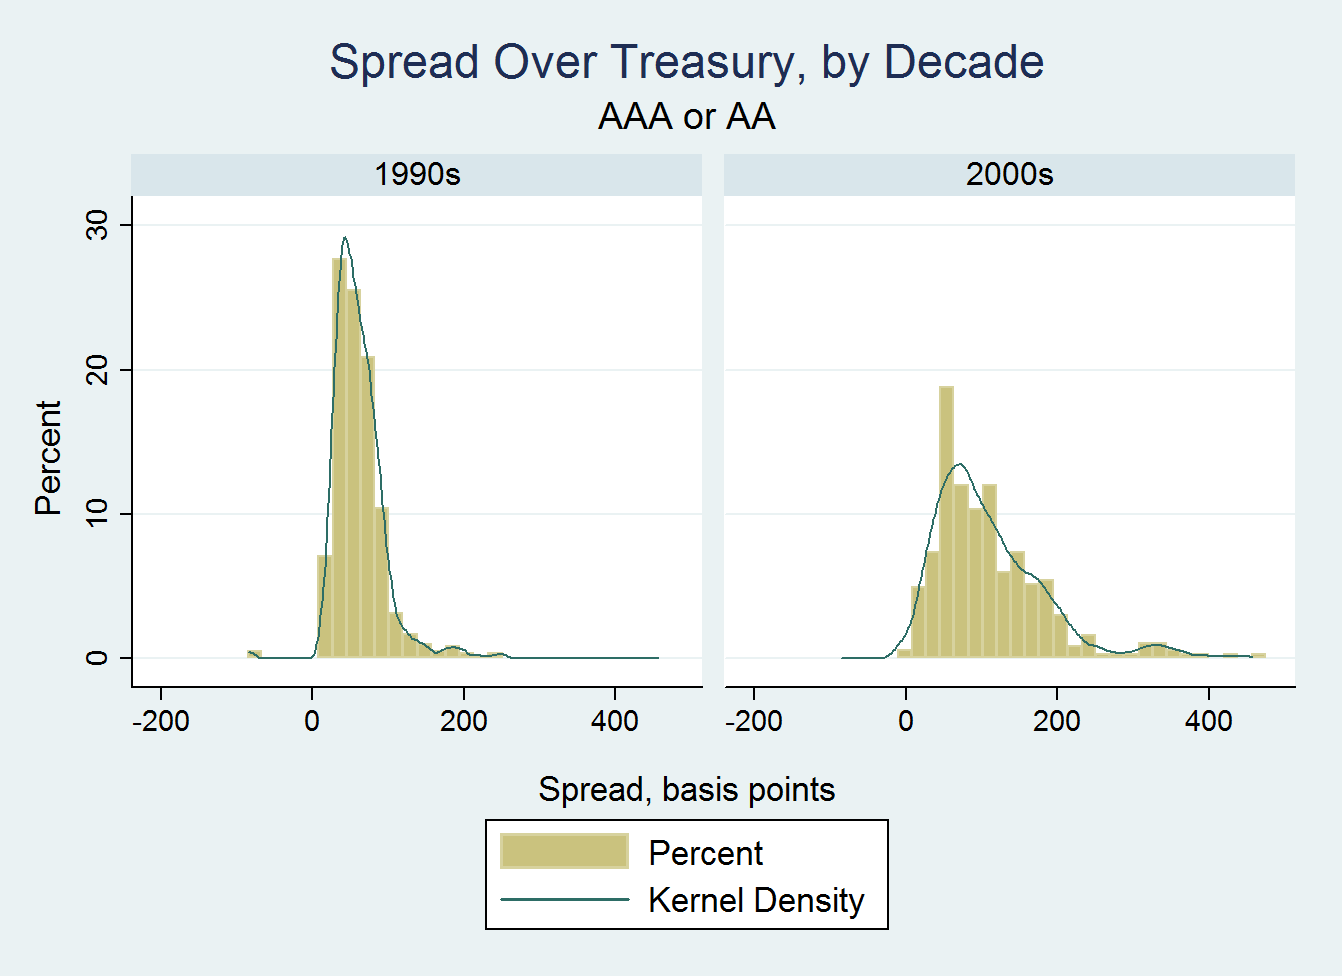
\includegraphics[width=\textwidth]{Spread_HiIG.png}
\caption{Spread over Treasury for AAA and AA bonds.}
\label{fig:spdHI}
\end{figure}

\begin{figure}[ht]
\centering
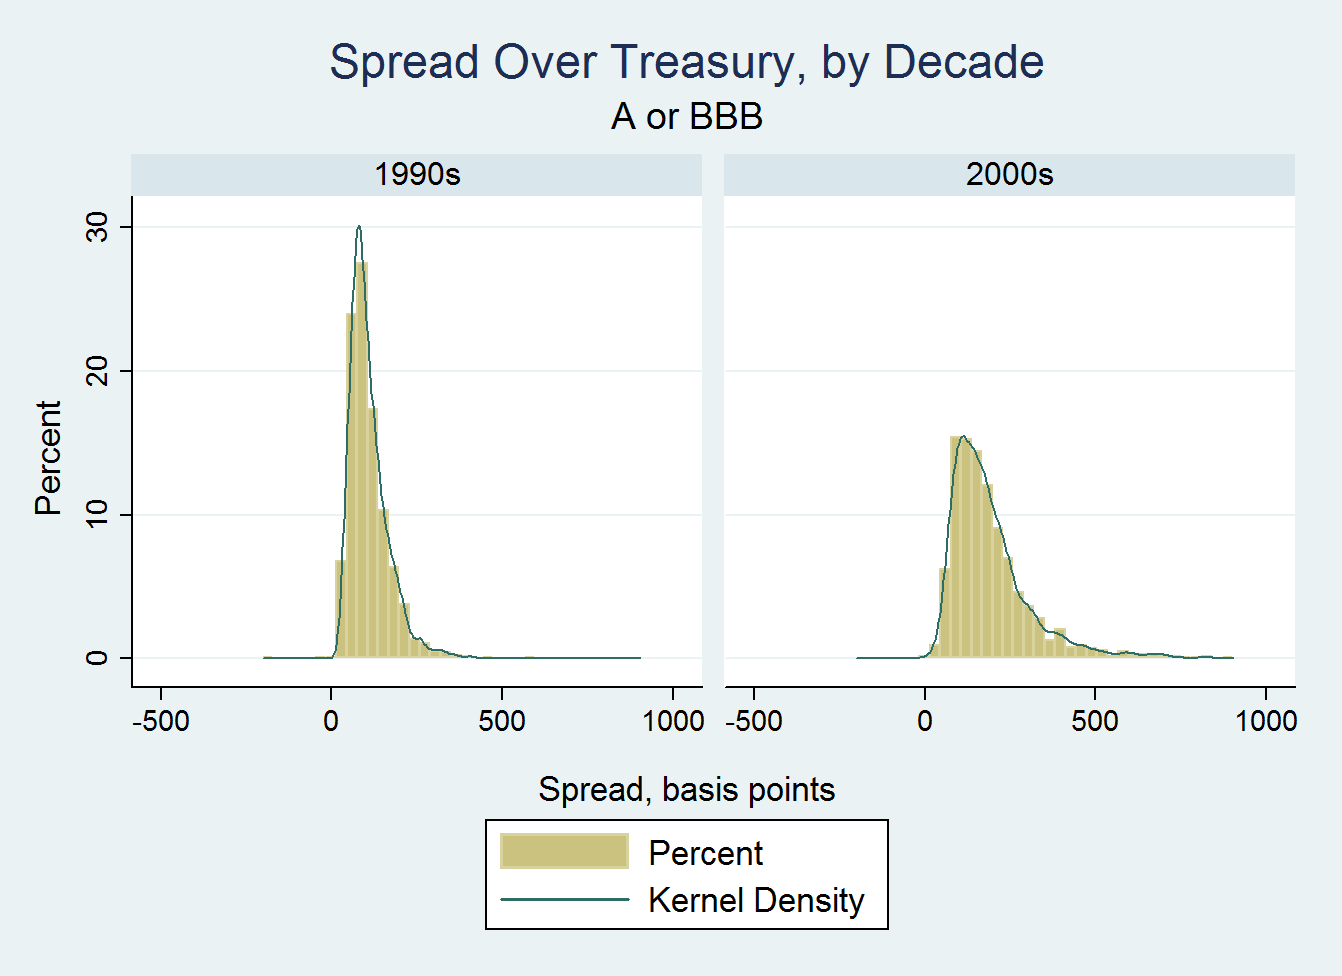
\includegraphics[width=\textwidth]{Spread_LoIG.png}
\caption{Spread over Treasury for A and BBB bonds.}
\label{fig:spdLO}
\end{figure}

\begin{figure}[ht]
\centering
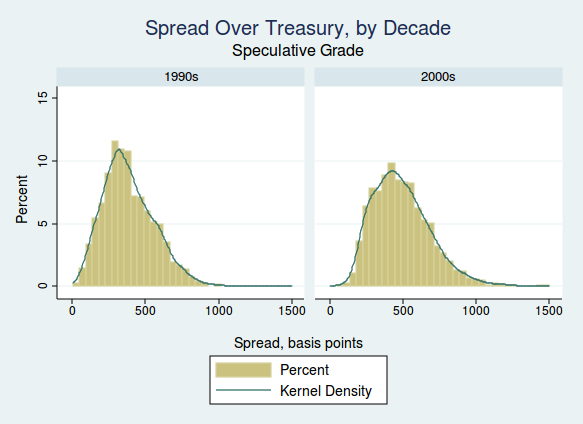
\includegraphics[width=\textwidth]{Spread_SG.png}
\caption{Spread over Treasury for BBB or lower bonds.}
\label{fig:spdSG}
\end{figure}

One concern is that the increasing dispersion is simply caused by an increasing mean, as one consequence of this is an increase in the standard deviation. As the coefficient of variation is immune to these perturbations it is more suited for this analysis. Therefore, to further substantiate the aforementioned pattern I calculate the coefficient of variation for each rating class and period as defined in Table~\ref{tab:sample}. I construct 95\% confidence intervals to determine whether any change in the coefficient of variation is statistically significant. The method applied can be found in Appendix (\ref{app:cov}). The result of this approach can be seen in Figure~\ref{fig:cov}. There is a large, statistically significant, increase in the coefficient of variation over the sample period in both the AAA and AA (which increased by 56\%) and the A and BBB (29\%) rating classes. Curiously, there is also a statistically significant decrease in the speculative grade rating class (26\%), though this disappears by the end of the sample period.

\begin{figure}[ht]
\centering
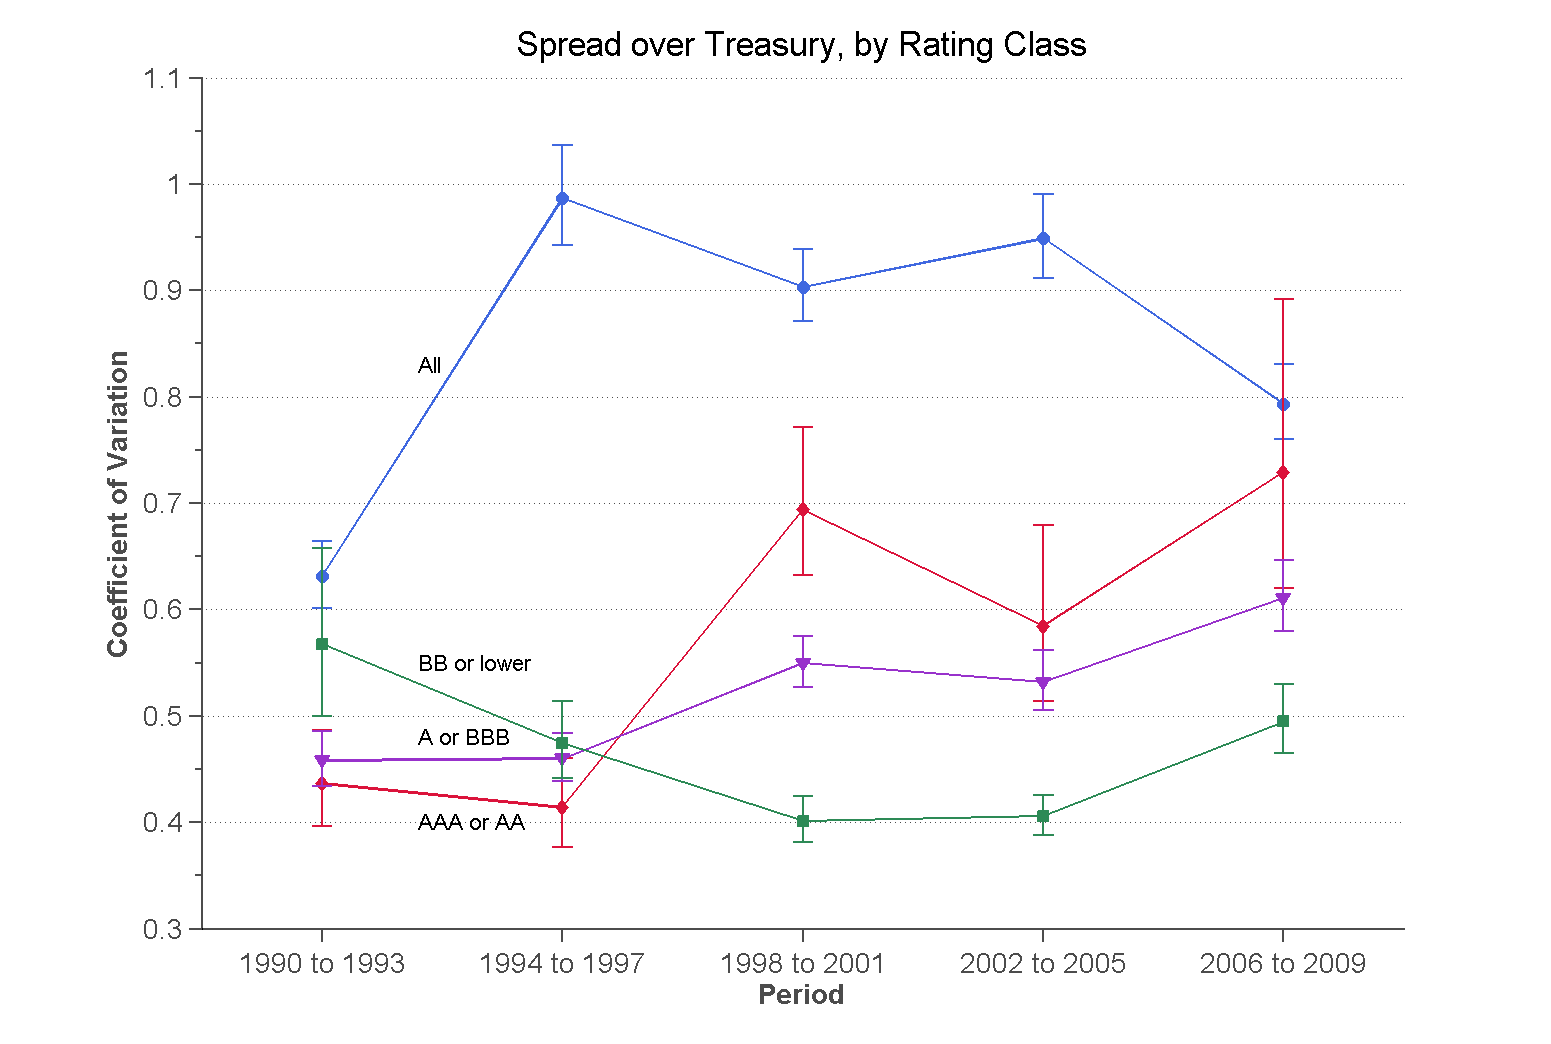
\includegraphics[width=\textwidth]{CVCI.png}
\caption{Coefficient of variation with 95\% confidence intervals, by rating class.}
\label{fig:cov}
\end{figure}

\section{Discussion}
\label{sec:dis}

In the wake of the 2007-2009 financial crisis, previous efforts to regulate capital markets have been questioned. A significant part of this scrutiny has been directed towards credit rating agencies (CRAs) and their role in mispricing risk. Though CRA behaviour has been studied in the context of other asset markets, the corporate bond market has been neglected. This paper is a step towards understanding the corporate bond market, specifically how firms behave when investors use both credit ratings and public information to make investment decisions and price bonds.

As public information has proliferated, its usefulness to investors has increased. Investors can now place more weight on this information as they evaluate firms. It is costly for firms to comply with the requirements of the CRAs as they improve their rating, whereas public information is provided without cost. Thus, firms are able to convey their creditworthiness at a reduced cost if investors use relatively more public information to make their invesment decisions and if the market price of their debt is determined in part by both credit ratings and public information.

I construct a model that captures the role of credit ratings and public information in the corporate bond market to provide an explanation of the ratings distribution shift. Proposition~(\ref{pr:pi}) states that firms will devote less resources to improving their credit rating as public information proliferates. This leads to the main result of the paper, Proposition~(\ref{pr:dist}), which shows that the number of firms with the highest rating will decrease, while the number of firms with mediocre and low ratings increase, when information proliferates. Thus, the change in the rating distribution of the model matches that in the data, lending creedence to proposed mechanism.

The shift in the credit ratings distribution is drastic. There has been a 70\% decrease in the number of AAA or AA rated firms, while the number of A or BBB rated firms has increased by 77\% and the number issuing speculative debt has increased by 129\%. This stark shift away from the top ratings towards the lower end of the rating distribution cannot be explained by changes in the leverage ratios of firms, nor can it be explained by mergers or changing CRA standards. 

Proposition~(\ref{pr:sprd}) states that, as the accuracy of public information increases, so too will the dispersion of interest rates within a rating group. The intuition for this result is straightforward: as investors now learn more about firms through public information they are able more accurately price debt above the accuracy provided by credit ratings. Using new data, I show that this is indeed the case for investment grade debt over the last 20 years. The coefficient of variation has increased by 56\% for AAA or AA rated debt and by 29\% for A or BBB rated debt. This dramatic increase in price dispersion is previously undocumented. 

As certain large investors are required to purchase highly rated debt or have lower capital requirements for investment grade debt holdings (as opposed to speculative), it is necessary for many firms to attain an investment grade credit rating to gain access to this segment of the market. Firms can also comply with CRA standards to improve their rating as this will lower their borrowing costs. This is costly, however, and as public information has become more reliable firms need no longer improve their credit rating to lower their borrowing cost. 

Understanding how firms use credit ratings is important as regulation of the credit rating agencies has become a pressing policy issue following the financial crisis of 2007-2009. To this point, the Dodd-Frank Act mandates the creation of an Office of Credit Ratings to enhance regulation of these agencies.\footnote{The official name of this act is `The Dodd-Frank Wall Street Reform and Consumer Protection Act.'} Much of this enhanced regulation will increase the bureaucratic burden of issuing a rating, the cost of which may be passed on to firms. If this comes to pass, my research suggests that firms will devote fewer resources to ratings, further lowering the reliability of credit ratings. 

Recognizing this behaviour is integral to understanding capital markets. Regulatory changes, such as the Dodd-Frank Act, which do not take this channel into account risk being ineffective, or worse, counter-productive. Also, the credit rating distribution is used by some as a measure of the aggregate riskiness of firms in the economy. In this paper I show that firms need not be riskier for the ratings distribution to shift towards lower ratings.

\section{Conclusion}
\label{sec:con}
This paper in part seeks an to answer the question ``why are the highly rated firms disappearing?'' The change in the distribution of firm ratings has been dramatic and has not thus far been documented in the academic literature. Possible explanations for this pattern, such as evolving credit rating agency standards, more highly levered firms, and firms merging, are explored and rejected. 

Instead I propose a mechanism that captures the increase in the proliferation of firm information. Investors no longer rely solely on credit ratings to relay firm information and firms need no longer devote resources to unproductive ratings activities. Thus the demand for high ratings is lessened from both investors and firms, a story consistent with the changes purported by the financial press. However, due to regulations that require certain types of investors to hold only investment grade assets, credit ratings retain a certain value. Considering this, it is the value of the highest ratings relative to other investment grade ratings that has diminished.

\newpage

\nocite{*}
\bibliographystyle{plain}
\bibliography{AAAbiblio}

\newpage

\appendix
\section{Appendix}
\subsection{Confidence Intervals on the Coefficient of Variation}
\label{app:cov}

Suppose random variable $X$ is distributed log-normal with mean $\mu$ and standard deviation $\sigma$. We would like to contruct a confidence interval on the coefficient of variation, $CV=\sqrt{Var(X)}/E(X)$. Helpfully, the coefficient of variation for a random variable distributed log-normal does not depend on the mean and can be entirely characterized by the variance.

Begin by determining the theoretical or ``true'' test statistic. The following are properties of log-normal distributions:
\begin{align}
E(X) & =  \exp(\mu+\frac{1}{2} \sigma^{2}) \\
Var(X) & =  \exp(2\mu + \sigma^{2})(\exp(\sigma^{2})-1) \\
\label{eq:cv} CV & = \sqrt{\exp(\sigma^{2})-1}.
\end{align}
Now, let $Y=\ln X$. Random variable $Y$ is distributed $N(\mu,\sigma^{2})$ and the test statistic for $\sigma^{2}$ is:
\begin{align*}
\frac{(n-1)s^{2}}{\sigma^{2}} & \sim \chi^{2}_{n-1}.
\end{align*}
The lower and and upper bounds can be defined as follows:
\begin{align*}
a_{L}&\equiv\frac{(n-1)s^{2}}{F_{\chi^{2}}(n-1)^{-1}(1-\alpha/2)}\\
a_{U}&\equiv\frac{(n-1)s^{2}}{F_{\chi^{2}}(n-1)^{-1}(\alpha/2)}
\end{align*}
Where $F_{\chi^{2}}(n-1)^{-1}(1-\alpha/2)$ is the cumulative distribution function for a chi-squared distribution with $n-1$ degrees of freedom. 

Using these bounds on $\sigma^{2}$ and equation~(\ref{eq:cv}), the following is a $1-\alpha$ confidence interval for the coeffecient of variation of $X$:
\begin{align}
[ \sqrt{\exp(a_{L})-1},\sqrt{\exp(a_{U})-1} ].
\end{align}
In order to compute the $(1-\alpha)$\% confidence interval of the coefficient of variation, all that is needed is the sample size, $n$, and the sample variance, $s^{2}$.

\subsection{Proposition~(\ref{pr:pi}): conditional distributions}
\label{app:pr:pi}
Show how $Pr\{\theta|\kappa,\nu\}$ changes with $\omega$.

\subsection{Proof of Proposition~(\ref{pr:sprd})}
Sketch:

$R^{*}(\kappa,H)$ decreasing in $\omega$.

$R^{*}(\kappa,L)$ increasing in $\omega$.

Therefore $R^{*}(\kappa,L)-R^{*}(\kappa,H)$ increasing in $\omega$.

\end{document}


%%%%%%%%%%
%old intro material
% Considering the value of a credit rating, a natural question arises: why are the highly rated firms disappearing? The topic was originally discussed in the financial press, from which three answers have been suggested. The first is that investors simply have a larger appetite for risk and are more willing to purchase corporate bonds that are not as safe as AAA or AA. The second answer is that firms find it too costly to maintain high ratings and are choosing asset and liability allocations that result in lower ratings. The third reason suggested by financial newspapers is that investors no longer place much stock in corporate bond ratings. I argue that these three reasons are essentially the same. Firms will lower their rating and reduce the associated costs if they are able to sell their debt at this new, lower, rating. This would be possible if the demand for lower investment grade bonds has increased relative to high investment grade bonds. The mechanism I propose is in the spirit of the answers suggested by the financial press, but the change is fundamental. As investors are able to rely on public sources of firm information, there is lower demand for ratings from both investors \emph{and} firms.

% Furthermore, these three potential answers are not entirely satisfying as they do not identify a fundamental reason for the shift in behaviour. They do, however, indicate that firms no longer rely on high ratings to sell their debt.

% The mechanism I propose is in the spirit of the answers suggested by the financial press, but the change is fundemental. As investors are able to rely on public sources of firm information, there is lower demand for ratings from both investors \emph{and} firms. By constructing a model that captures this change, I show that the resulting shift in the ratings distribution matches the shift observed in the data. Furthermore, the model predicts an increase in the within rating price dispersion for investment grade bonds. Using new data, I document this pattern as well.

% By constructing a model that captures this change, I show that the resulting shift in the ratings distribution matches the shift observed in the data. Furthermore, the model predicts an increase in the within rating price dispersion for investment grade bonds. Using new data, I document this pattern as well.

% To this point:
% \begin{quote}
% ``Scores of big companies have lost their AAA status in recent years as it became seen in board rooms as more of a straitjacket than a path to riches.''\attrib{Eric Dash, New York Times, August 2, 2011}
% \end{quote}
% Put slightly differently, firms are no longer willing to pay the cost to achieve these high ratings. My conjecture begins with the point that these ratings have value as a signal of firm ``quality'' in the sense that they provide investors with information about the future performance of the firm, in addition to the rating's primary role as an indicator of the firm's credit worthiness. As the proliferation of information has increased, firms no longer rely on a rating as a signal of its overall quality because investors now learn about firms through other channels which are costless to the firm. These channels include SEC 10K filings, which contain pertinent financial data from public firms and are now provided electronically, and also include media such as the Wall Street Journal Online and Bloomberg. In short, investors have direct access to firm information and firms no longer need to rely on a credit rating as a signal of their type.